\chapter{Backferment Brot}
\todo{Erstellung Grundansatz}
\section{Dinkelvollkornbrot} \index{Brot!Dinkel}\index{Vollkorn!Brot}\index{Backferment!Brot}
\subsection*{Allgemeines}

\begin{tabular}{lrl}
    Gesamtzeit          & 16 --  24 & Stunden           \\
    Vorteig erstellen   &        10 & Minuten           \\
    Vorteig             &  12 -- 16 & Stunden           \\
    Brühstück           &        10 & Minuten           \\
    Gehzeit             &        30 & Minuten           \\
    Hauptteig erstellen &        10 & Minuten           \\
    1. Gehzeit          &        50 & Minuten           \\
    2. Gehzeit          &  30 -- 50 & Minuten           \\
    Backzeit            &         1 & Stunde \\ 
    && \cite[Seite 159 ]{Pokorny2016}
\end{tabular} 

\subsection*{Zutaten}

\subsubsection*{Vorteig}
\begin{tabular}{lrr}
    Dinkelvollkornmehl                  & 150 &  g \\
    lauwarmes Wasser (ca. 40 $^\circ$C) & 150 & ml \\
    Grundansatz                         &  10 &  g \\
    Backferment                         &   3 &  g
\end{tabular} 

Grundansatz mit Backferment in etwas Wasser auflösen, restliches Wasser zugeben und mit dem Vollkornmehl gründlich vermengen. Bedeckt bei ca. 24 $^circ $C mindestens 12 Stunden stehen lassen. 

\subsubsection*{Brühstück}
\begin{tabular}{lrr}
    Dinkelvollkornmehl                  & 100 (150) &  g \\
    kochendes Wasser  & 180 (280) & ml \\
\end{tabular} 

Mehl mit dem Wasser (genau abmessen) über brühen. Gut durchkneten. Das Brühstück soll ziemlich fest, aber nicht hart sein. Falls nötig nochmal etwas kochendes Wasser einarbeiten. Bedeckt ca. 30 Minuten ausquellen lassen.  

\subsubsection*{Hauptteig}
\begin{tabular}{lrr}
    Dinkelvollkornmehl & 250 &  g \\
    sehr warmes Wasser (ca. 45 $^\circ$C) & 150 (50) & ml \\
    Hefe   & 2-3          &   g \\
    Salz        & 10 & g \\
\end{tabular} 

\subsection*{Zubereitung}

\begin{enumerate}
    \item Den Vorteig mit dem Brühstück homogen vermengen.
    \item Zum Vorteig das gesalzene Vollkornmehl hinzugegeben und vermengen. Hefe in Wasser auflösen und nach und nach Wasser hinzugeben. Der Teig soll mittelfest sein. Zur Not etwas warmes Wasser oder Mehl hinzugeben. 
    \item Bedeckt 40 Minuten stehen lassen. Durchkneten, nach Belieben Körner (Sonnenblumen schmeckt gut, ca. 100g) hinzugeben und in warme gefettete Backformen  (oder Garkörbchen) legen.
    \item Bedeckt weitere 40 Minuten stehen lassen. Backofen vorheizen ($ 220\;^{circ} $C, Umluft $ 200\;^{circ} $C) und Wasserschüssel einstellen. Teigstücke an der Oberfläche befeuchten und ca. eine Stunde backen.    
\end{enumerate}  

\section{Weizen-Roggen-Vollkorn} \index{Brot!Weizen-Roggen}\index{Brot!Roggen}\index{Brot!Weizen}\index{Vollkorn!Brot}\index{Backferment!Brot}
\subsection*{Allgemeines}
\begin{tabular}{lrl}
    Gesamtzeit          & 16 --  24 & Stunden                       \\
    Vorteig erstellen   &        10 & Minuten                       \\
    Vorteig             &  12 -- 16 & Stunden                       \\
    Hauptteig erstellen &        10 & Minuten                       \\
    1. Gehzeit          &        50 & Minuten                       \\
    2. Gehzeit          &  30 -- 50 & Minuten                       \\
    Backzeit            &         1 & Stunden                       \\
    &           & \cite[Seite 66 ]{Pokorny2016}
\end{tabular} 
\subsection*{Zutaten}

\subsubsection*{Vorteig}
\begin{tabular}{lrr}
    Weizenvollkornmehl                  & 100 &  g \\
    Roggenvollkornmehl                  & 100 &  g \\
    lauwarmes Wasser (ca. 40 $^\circ$C) & 200 & ml \\
    Grundansatz                         &  10 &  g \\
    Backferment                         &   2 &  g
\end{tabular} 

Grundansatz mit Backferment in etwas Wasser auflösen, restliches Wasser zugeben und mit dem Vollkornmehl gründlich vermengen. Bedeckt bei ca. 24 $^{\circ} $C mindestens 12 Stunden stehen lassen. 

\subsubsection*{Hauptteig}
\begin{tabular}{lrr}
    Weizenvollkornmehl & 150 &  g \\
    Roggenvollkornmehl & 150 &  g \\
    sehr warmes Wasser (ca. 45 $^\circ$C) & 175 & ml \\
    Hefe   & 2-3          &   g \\
    Salz        & 10 & g \\
\end{tabular} 

\subsection*{Zubereitung}

\begin{enumerate}
    \item Zum Vorteig die gesalzenen Vollkornmehle hinzugegeben und vermengen, Hefe in Wasser auflösen und nach und nach Wasser hinzugeben.
    \item Bedeckt 50 Minuten stehen lassen. Durchkneten, nach Belieben Körner (Sonnenblumen schmeckt gut, ca. 100~g) hinzugeben und in warme gefettete Backformen  (oder Garkörbchen) legen.
    \item Bedeckt weitere 40 Minuten stehen lassen. Backofen vorheizen ($ 220\;^{\circ} $C, Umluft $ 200\;^{\circ} $C) und Wasserschüssel einstellen. Teigestücke an der Oberfläche befeuchten und ca. eine Stunde backen.    
\end{enumerate}  

\section{Weizen-Hafer-Vollkorn} \index{Brot!Weizen-Hafer}\index{Brot!Hafer}\index{Hafer}\index{Brot!Weizen}\index{Vollkorn!Brot}\index{Backferment!Brot}
Der Hafer sorgt für ein mildes gut schmeckendes Brot. Das Ausquellen ist unbedingt erforderlich!
\subsection*{Allgemeines}
\begin{tabular}{lrl}
    Gesamtzeit          & 16 --  24 & Stunden                       \\
    Vorteig erstellen   &        10 & Minuten                       \\
    Vorteig             &  12 -- 16 & Stunden                       \\
    Hauptteig erstellen &        10 & Minuten                       \\
    Ausquellen          &        15 & Minuten                       \\
    1. Gehzeit          &        40 & Minuten                       \\
    2. Gehzeit          &  30 -- 40 & Minuten                       \\
    Backzeit            &  50 -- 60 & Minuten                       \\
    &           & \cite[Seite 151 ]{Pokorny2016}
\end{tabular} 
\subsection*{Zutaten}

\subsubsection*{Weizen-Hafer-Mischung}
\begin{tabular}{lrr}
    Hafervollkornmehl                  & 150 &  g \\
    Weizenvollkornmehl                 & 350 &  g \\
\end{tabular} 

\subsubsection*{Vorteig}
\begin{tabular}{lrr}
    Weizen-Hafer-Mischung               & 150 &  g \\
    lauwarmes Wasser (ca. 40 $^\circ$C) & 150 & ml \\
    Grundansatz                         &  10 &  g \\
    Backferment                         &   3 &  g
\end{tabular} 

Grundansatz mit Backferment in etwas Wasser auflösen, restliches Wasser zugeben und mit dem Vollkornmehl gründlich vermengen. Bedeckt bei ca. 24 $^{\circ} $C mindestens 12 Stunden stehen lassen. 

\section{Verdoppelung \Gls{Sauerteig}}\index{Sauerteig!Zubereitung}\label{sec:Sauerteig}
Mein Sauerteig ist ein umgezogener Lievito Madre.  

\begin{enumerate}
    \item 100\;g Anstellgut werden mit 50\; g Roggenvollkornmehl und 50\;g Roggen 1150 gemischt (nicht lange kneten). 
    \item Dann bei ca. 29 -- 31 Grad 3-4 reifen lassen.
    \item Jetzt die Hälfte des Sauerteigs aufheben (Kühlschrank) für das nächste mal Backen und mit der anderen Hälfte ihr Brot backen.
    \item Braucht man mehr Brot, so kann man den Vorgang mehrmals wiederholen.
\end{enumerate}

\chapter{Sauerteig}

\section{Verdoppelung \Gls{LievitoMadre}: Hartie}\index{Lievito Madre!Zubereitung}\label{sec:Lievito Madre}

\begin{enumerate}
    \item 100\;g Anstellgut wird 50\;g Wasser gemischt und dann ca. 10 Minuten ruhen lassen.  
    \item 50 g Semola und 50 g Tipo 0 zugegeben und gut durchkneten.
    \item Dann bei ca. 29 -- 31 Grad 3-5 Stunden reifen lassen.
    \item Braucht man mehr Lievito Madre, so kann man den Vorgang mehrmals wiederholen.
\end{enumerate}

\section{Sauerteig Roggenbrot} \index{Brot!Roggen}\index{Brot!Sauerteig}\index{Sauerteig}
\subsection*{Allgemeines}
\begin{tabular}{lrl}
	Gesamtzeit          & 17 --  24 & Stunden                        \\
	Vorteig erstellen   &        10 & Minuten                        \\
	Vorteig             &  12 -- 16 & Stunden                        \\
	Hauptteig erstellen &        10 & Minuten                        \\
	1. Gehzeit          &         2 & Stunden                        \\
	2. Gehzeit          &         2 & Stunder                        \\
	Backzeit            &  50 -- 60 & Minuten                        \\
\end{tabular} 
\subsection*{Zutaten}
\begin{tabular}{lrr}
	Sauerteig                        & 300 &  g \\
	Roggenmehl                       & 500 &  g \\
	warmes Wasser (ca. 40 $^\circ$C) & 375 & ml \\
	Hefe                             & 2-3 &  g \\
	Salz                             &   3 & TL
\end{tabular} 


\subsection*{Zubereitung}

Für die Zubereitung von Sauerteig siehe \vref{sec:Sauerteig}.

\begin{enumerate}
	\item Den Natursauerteig in eine Schüssel geben und mit den	restlichen Zutaten zu einem	glatten Teig verarbeiten. In der Maschine nur langsam kneten.
	\item Den Teig mit Mehl bedeckt ca.2 Stunden bei Zimmertemperatur ruhen lassen.	
	\item Kurz durchkneten und in eine Brotform geben. Erneut 2 Stunden Ruhe.
	\item Backofen vorheizen ($ 250\;^{\circ} $C) und Wasserschüssel einstellen. Teige einschneiden, mit Wasser besprühen und bei fallender Hitze (Ende bei $180\;^{\circ}$) abbacken.
\end{enumerate}   

Man kann auch 20\% des Roggenmehls durch Weizenmehl oder Dinkelmehl ersetzen. Das ergibt ein lockeres milderes Brot.



\section[Ciabatta / Pain Paillasse]{Ciabatta / Pain Paillasse \textmd{(siehe \cite{HollensteinerCiabatta}})}  \index{Brot!Weizen}\index{Brot!Lievito Madre}\index{Ciabatta}\label{sec:brot:Ciabatta:LM}

\subsection*{Zeitplan}
\begin{tabular}{ r @{ Uhr \phantom{bla} } l}
    \toprule
    \multicolumn{1}{c @{\phantom{ bla }}}{Zeit} & \multicolumn{1}{@{}l}{Aktion}      \\ \midrule
    00:00                                & \Gls{Autolyse}                    \\
    00:15                                & \Gls{Hauptteig}                    \\
    00:35                                & \Gls{Stockgare}                    \\
    03:35                                & \Gls{Formen} \\
    03:45								 & \Gls{Stueckgare}     \\ \midrule
    \multicolumn{2}{c}{Wurzelbrot}   \\
    04:00 &   \Gls{Backen} \\ 
    04:20 & fertig\\ \midrule
    \multicolumn{2}{c}{Ciabatta}   \\
    04:30 &   \Gls{Backen} \\
    04:55 &  fertig\\ \bottomrule
\end{tabular}

\subsection*{Zutaten}

\begin{tabular}{r l}
    \toprule
    100 g & Lievito Madre TA 150 \\ \midrule
    230 g & Tipo 0               \\
    320 g & Wasser (kühl)        \\ \midrule
    230 g & Weizenmehl  550er    \\
    310 g & Wasser (kühl)        \\ \midrule
    100 g & Hartweizenmehl       \\
      8 g & Salz                 \\
      8 g & Olivenöl             \\
    3,5 g & Frischhefe           \\ \bottomrule
\end{tabular}

\subsection*{Zubereitung}
\begin{enumerate}
   \item Alle Zutaten in den Kneter geben. Mit dem Flachschlägerhaken  3 Minuten langsam rühren, bis alles zu einem Brei verrührt ist.
   \item 10 Minuten Pause.
   \item Dann auf Stufe 2-3 schalten und den Flachschlägerhaken so lange rühren lassen, bis sich der Teig komplett von der Schüssel löst. Das hat bei mir etwa 10-12 Minuten gedauert.
   \item Den Teig in eine Teigwanne geben und mindestens 2 1/2 bis 3 Stunden reifen lassen. Ggf. noch länger. Während der ersten 90 Minuten zweimal dehnen und falten. Der Teig sollte sich gut verdreifacht haben vom Volumen und stark von Gasblasen durchzogen sein.
   \item Auf die gut bemehlte Arbeitsfläche kippen und die Rückseite bemehlen. Wenn die Teigwanne rechteckig war, von den kurzen Seiten her rasch und selbstsicher zwei Stücke abstechen. Mit den bemehlten Händen greifen und auf ein Backpapier legen. Dort dann mit raschen Handbewegungen die Teigstücke 3 – 4 mal (nicht zu oft) um sich selbst drehen, sodass die Wurzelform entsteht.
   \item Wenn es Ciabatta werden sollen, lediglich abstechen und auf das Backpapier befördern. Die Wurzelbrote noch etwa 15 Minuten entspannen lassen und dann sofort backen. Lässt man sie länger reifen, verwischen die Furchen zu stark. Ciabattateiglinge können noch gut und gerne 45 Minuten Stückgare vertragen, dann werden sie innen noch luftiger.
   \item Bei 250° in den gut vorgeheizten Ofen geben und sofort schwaden. Bei konstant 250° kräftig dunkel ausbacken
\end{enumerate}
 
\section[Ciabattine] {Ciabattine \textmd{(siehe {SonjaBauer2023})}} \index{Brot!Weizen}\index{Brötchen!Lievito Madre}
\begin{tabular}{ r @{ Uhr \phantom{bla} } l}
    \toprule
    \multicolumn{1}{c @{\phantom{ bla }}}{Zeit} & \multicolumn{1}{@{}l}{Aktion}     \\ \midrule
    00:00                                       & \Gls{Autolyse}                    \\
    01:00                                       & \Gls{Hauptteig}                   \\
    01:15                                       & \Gls{Stockgare}  Raumtemperatur   \\
    05:15                                       & \Gls{Formen} und \Gls{Stueckgare} \\
    05:30                                       & \Gls{Vorheizen}                   \\
    06:00                                       & \Gls{Backen}                      \\
    06:20                                       & fertig                            \\ \bottomrule
\end{tabular}

\subsection*{Zubereitung}

\subsubsection*{\Gls{Autolyse}}
\begin{tabular}{r l}
    270 g & kühles Wasser\\
    350 g & Tipo 00
\end{tabular}\\


\section[Focaccia]{Focaccia  \textmd{(siehe \cite[173]{SonjaBauer2021} und \cite{sonjaFocaccia})} }  \index{Brot!Weizen}\index{Brot!Lievito Madre}\index{}

%\begin{figure}[H]
%    \centering
%    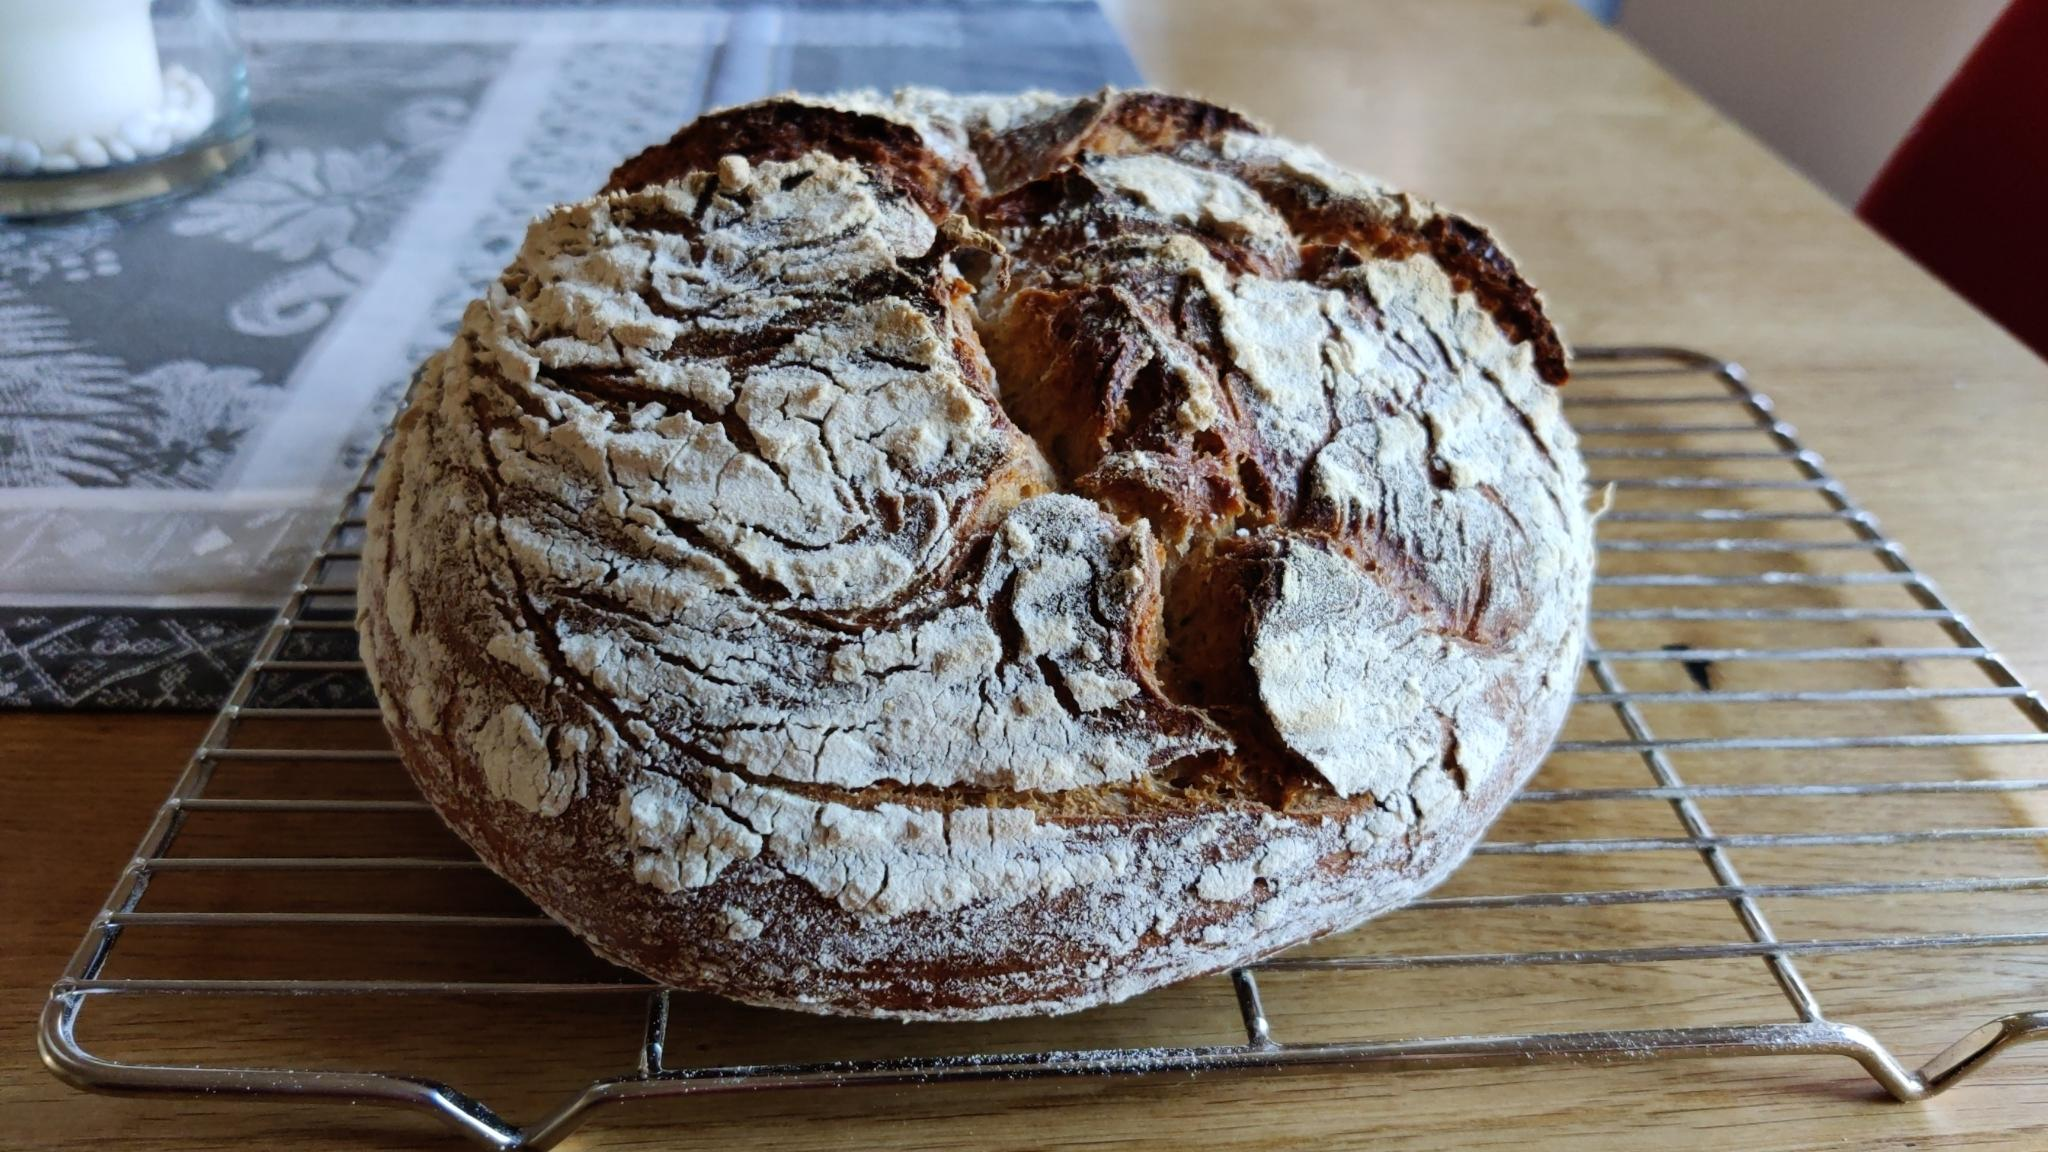
\includegraphics[width=0.7\linewidth]{Bilder/JulesSchwester}
%    \caption{Focaccias aus zwei Rezepten}
%    \label{fig:auffrischbrotJulesSchwester}
%\end{figure}

\subsection*{Zeitplan}
\begin{tabular}{ r @{ Uhr \phantom{bla} } l}
    \toprule
    \multicolumn{1}{c @{\phantom{ bla }}}{Zeit} & \multicolumn{1}{@{}l}{Aktion}   \\ \midrule
    00:00                                       & \Gls{Autolyse}                 \\
    00:30                                       & \Gls{Hauptteig}                 \\
    00:45                                       & \Gls{Stockgare}  Raumtemperatur   \\
    06:45                                       & \Gls{Stockgare}  Kühlschrank mindestens  \\
    12:45                                       & \Gls{Formen} und \Gls{Stueckgare}     \\
    15:45                                       & \Gls{Backen}                          \\
    16:20                                       & fertig                  \\ 
    \bottomrule
\end{tabular}


\subsection*{Zubereitung}

\subsubsection*{\Gls{Autolyse}}
\begin{tabular}{r l}
    350 g & kühles Wasser\\
    500 g & Tipo 00
\end{tabular}\\

Kurz, aber gründlich vermischen.
Für 30 Minuten abgedeckt quellen lassen.

\subsubsection*{\Gls{Hauptteig}}
\begin{tabular}{r l}
           + & Autolyse                               \\
        50 g & Lievito Madre (maximal 12 Stunden alt) \\
         5 g & Honig                                  \\
        15 g & Olivenöl                               \\
        20 g & Salz                                   \\
         2 g & Hefe                                   \\
         2-3 & Knoblauchzehe                          \\
    1 Zweig & Rosmarin gehackt
\end{tabular}\\

Lievito Madre (LM), Hefe und Honig zur Autolyse geben und für 10 Minuten mit geringer Stufe kneten. Salz, Knoblauch, Rosmarin und Olivenöl zugeben, für 3–5 Minuten mit höherer Stufe aus kneten.



\subsubsection*{\Gls{Stockgare}}
Den Teig auf leicht geölter Backfolie in Teigwanne bei Raumtemperatur abgedeckt etwa 10-12 Stunden Gare (erst 6-8 Stunden und dann in den Kühlschrank) stellen. Nach 60 und 120 Minuten dehnen und falten.

\subsubsection*{Formen}
Backpapier/Dauerbackfolie auslegen. Den Teig darauf geben und mit den Händen etwas Olivenöl auf die Teigoberfläche auftragen. 
\subsubsection*{\Gls{Stueckgare}}
Locker abgedeckt für etwa 3 Stunden zur Gare stellen. Mit 40 g Olivenöl 40g Wasser und einem halben Teelöffel Salz mischen und bestreichen . Mulden eindrücken und belegen (Tomaten, Rosmarin und Oliven)

\subsubsection*{Backen}
Bei 230 Grad in den vorgeheizten Ofen. Dampfen. Nach 10 Minuten abdampfen und für weitere 20 Minuten auf 200 Grad reduzieren.


\section{Dinkel Karotten Brot}  \index{Brot!Dinkel}\index{Brot!Möhren}\index{Brot!Lievito Madre}\index{Brot!Kastenbrot}

\todo{Sonja Bauer 176 }
%HAUP T TEIG
%250–280 g Wasser, kühl
%( je nach Saftigkeit der Karotten)
%1 g
%Frischhefe
%0,8 g*
%Acerola-Pulver (optional)
%150 g
%Joghurt, kalt
%150 g
%Möhren, grob geraspelt
%10 g
%inaktives Backmalz/
%Honig
%500
%Dinkelvollkornmehl
%125 g
%gemischte Saaten**,
%geröstet
%12 g
%Salz
%10 g
%Rapsöl
%ZU S ÄT ZL I C H
%gemischte Saaten
%
%Hefe und Acerola-Pulver in dem Wasser auflösen.
%Danach alle Zutaten für den Hauptteig (außer Salz +
%Rapsöl) hinzufügen und für 8–10 Minuten mit geringer
%Stufe kneten. In den letzten 2 Minuten Salz und Rapsöl
%zugeben.
%O D E R : Für 5–6 Minuten bei geringer Stufe in der
%Küchenmaschine mit einem Rührelement mit Gummi-
%lippe mischen. In der letzten Minute Salz und Rapsöl
%zugeben.
%Ohne Hefe:
%Statt 1 g Frischhefe können 30 g vom Weizen-/Rog-
%gen-Anstellgut (ASG) oder Lievito Madre (LM) aus dem
%Kühlschrank ver wendet werden – das ASG/LM sollte
%sehr aktiv sein. Für 10–12 Stunden bei 22–24° C zur
%Stockgare stellen.
%
%IN DIE K A STENFORM GEBEN
%Den Teig in eine gefettete und mit reichlich Saaten ausgestreute/mit Dauerbackfolie ausge-
%legte Kastenform füllen. Teigoberfläche mit einem angefeuchteten Teigschaber glattstrei-
%chen und mit Saaten bestreuen. Die Kastenform ist gut zur Hälfte gefüllt.
%
%9 –1 1 S T D.
%2 0 –2 2° C
%S T Ü C KG A R E
%ZIEL: ca. 1 cm unter dem Rand
%Abgedeckt für 9–11 Stunden bei Raumtemperatur zur Gare stellen.
%Der Teig soll etwa knapp den Rand der Form erreichen.
%6 0 M IN .
%2 3 0° C
%2 0 0° C
%BACKEN
%Backofen rechtzeitig mit einem Backstahl oder Backstein auf 230° C
%Ober-/Unterhitze vorheizen.
%Für insgesamt 60 Minuten ohne Schwaden backen. Nach 10 Minuten die Temperatur auf
%200° C reduzieren. Für die letzten 10 Minuten aus der Form nehmen und zu Ende backen.


\section{Vollkornprotz}  \index{Brot!Dinkel}\index{Brot!Weizen}\index{Brot!Roggen}\index{Brot!Buttermilch}\index{Brot!Lievito Madre}\index{Brot!Roggensauerteig}\index{Brot!Kastenbrot}

\begin{figure}[H]
    \centering
    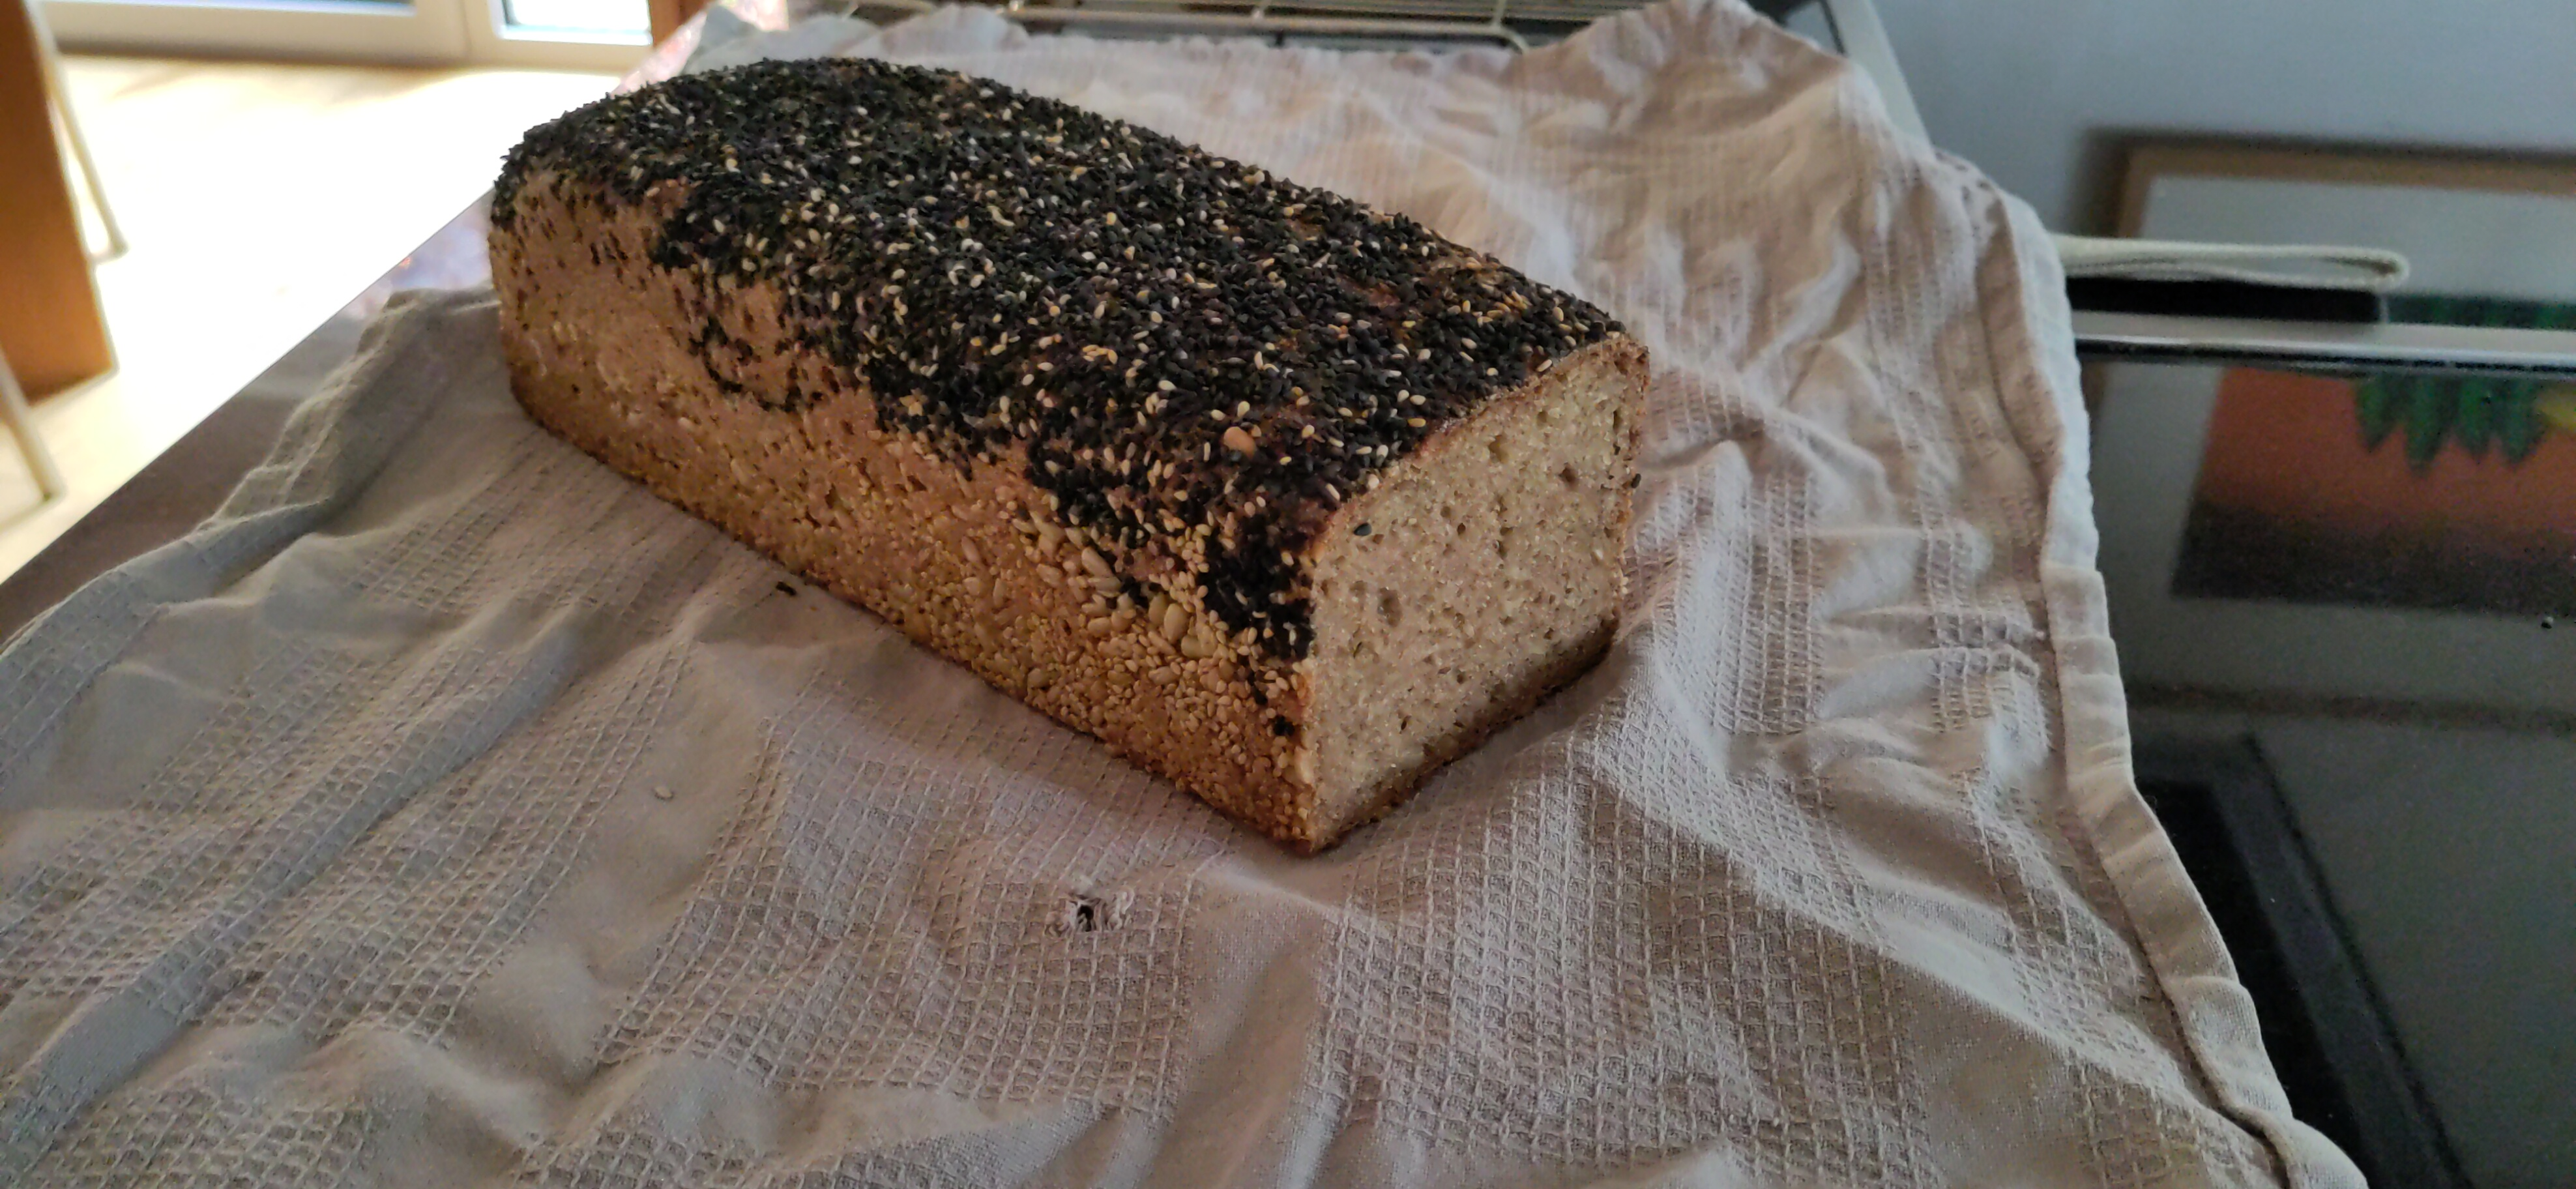
\includegraphics[width=0.7\linewidth]{Bilder/Vollkornprotz}
    \caption{Vollkornprotz mit schwarzem Sesam}
    \label{fig:vollkornprotz}
\end{figure}
 
 
\subsection*{Hauptteig}
\begin{tabular}{r l}
          40 g & Roggensauerteig oder Lievito Madre (+20 g Wasser) \\
         400 g & Buttermilch, kalt                                 \\
         140 g & Wasser, 40° C                                     \\
          10 g & Rübensirup                                        \\
         350 g & Weizenvollkornmehl                                \\
         100 g & Dinkelvollkornmehl                                \\
          50 g & Roggenvollkornmehl                                \\
         0,8 g & Acerola-Pulver                                    \\
          60 g & Sonnenblumenkerne, geröstet                       \\
          20 g & Sesam, geröstet                                   \\
          12 g & Salz                                              \\
          10 g & Olivenöl                                          \\
    zusätzlich & Sonnenblumenkerne und Sesam zum Streuen
\end{tabular}\\

\subsection*{Zubereitung}

\begin{enumerate}
    \item [\Gls{Hauptteig}]  Buttermilch und Wasser mischen. Danach alle Zutaten (das ASG/LM sollte sehr aktiv sein.) für den Hauptteig (außer Salz + Speiseöl) für 8–10 Minuten mit geringer Stufe kneten. Danach 2 Minuten schneller kneten, dabei Salz und Olivenöl zugeben. 
    \item [\Gls{Stueckgare}] 
    Den Teig in eine gefettete und mit reichlich Saaten ausgestreute Kastenform füllen. Teigoberfläche glattstreichen und mit Saaten bestreuen. Die Kastenform ist etwa zur Hälfte gefüllt.\\
    Für 10–12 Stunden bei 22–24° C (13–15 Stunden bei 21° C) zur Stockgare stellen. 
    \item[\GLS{Backen}]
    Backofen rechtzeitig mit einem Backstahl auf 230°C Ober-/Unterhitze vorheizen. Für insgesamt 60 Minuten ohne Schwaden backen. Nach 10 Minuten die Temperatur auf 200° C reduzieren. Für die letzten 10 Minuten aus der Form nehmen und zu Ende backen.
\end{enumerate}

\section[Urkornkasten]{Urkornkasten \textmd{(siehe \cite[188]{SonjaBauer2021})}}  \index{Brot!Urkornkasten} \index{Buttermilch} \index{Brot!Buttermilch}

\subsection*{Zeitplan}
\begin{tabular}{ r @{ Uhr \phantom{bla} } l}
    \toprule
    \multicolumn{1}{c @{\phantom{ bla }}}{Zeit} & \multicolumn{1}{@{}l}{Aktion} \\ \midrule
    00:00                                       & Anstellgut Roggen             \\
    04:00                                       & \Gls{Hauptteig}               \\
    04:15                                       & \Gls{Stueckgare}              \\
    14:45                                       & Vorheizen                     \\
    15:15                                       & \Gls{Backen}                  \\
    16:15                                       & fertig                        \\ \bottomrule
\end{tabular}

\subsection*{Zutaten}
Zweiter Wert für kleinere Backform (ca. 750 g)

\begin{tabular}{r l}
          30 / 22,5 g & aufgefrischt Roggensauerteig oder Lievito Madre (+15 g Wasser) \\
         250 / 187,5  g & Buttermilch                                                    \\
         300 / 225 g & Wasser, 40° C                                                  \\
          10 / 7,5 g & inaktives Backmalz                                             \\
         300 / 225 g & Dinkelvollkornmehl                                             \\
         100 / 75 g & Dinkelmehl  630                                                \\
          50 / 37,5 g & Roggenvollkornmehl                                             \\
          50 / 37,5 g & Waldtaudenroggenmehl                                           \\
          50 / 37,5 g & kernige Haferflocken                                           \\
         0,8 / 0,6 g & Acerola-Pulver                                                 \\
           3 / 2,25 g & Flohsamen                                                      \\
          30 / 22,5 g & Sonnenblumenkerne, geröstet                                    \\
          20 / 15 g & Sesam, geröstet                                                \\
          12 / 9 g & Salz                                                           \\
          10 / 7,5 g & Rapsöl                                                         \\
    zusätzlich & Haferflocken Sonnenblumenkerne und Sesam zum Streuen
\end{tabular}\\

\subsection*{Zubereitung}
\begin{enumerate}
    \item  [\Gls{Hauptteig}]  Wasser und Buttermilch mischen, Roggen-Anstellgut und das Acerola-Pulver darin auflösen. Danach alle Zutaten für den Hauptteig (außer Salz + Öl) hinzufügen und für 8–10 Minuten mit geringer Stufe kneten. In den letzten 2 Minuten Salz und Öl zugeben.
    \item [\GLS{Formen}] Den Teig in eine gefettete und mit Haferflocken, Sonnenblumenkerne und Sesam ausgestreute ausgelegte Kastenform füllen. Teigoberfläche mit einem angefeuchteten Teigschaber glattstreichen und mit Haferflocken, Sonnenblumenkernen und
    Sesam bestreuen. Die Kastenform ist etwa zur Hälfte gefüllt.
    \item [\Gls{Stueckgare}] Abgedeckt für 10–12 Stunden bei warmer Raumtemperatur (22–24° C) zur Gare stellen. Der Teig soll etwa knapp den Rand der Form erreichen.
    \item [\Gls{Backen}] Backofen rechtzeitig mit einem Backstahl oder Backstein auf 230° C Ober-/Unterhitze vorheizen. \\
    Für insgesamt 60 Minuten ohne Schwaden backen. Nach 10 Minuten die Temperatur auf
    200° C reduzieren. Für die letzten 10 Minuten aus der Form nehmen und zu Ende backen. 
\end{enumerate}



\section[Mischbrot 50/50]{Mischbrot 50/50 \textmd{(siehe \cite[130]{SonjaBauer2021})}}  \index{Brot!Mischbrot 50/50} \index{Malzbier} \index{Brot!vegan!Mischbrot}
%\begin{figure}[H]
%%    \centering
%%    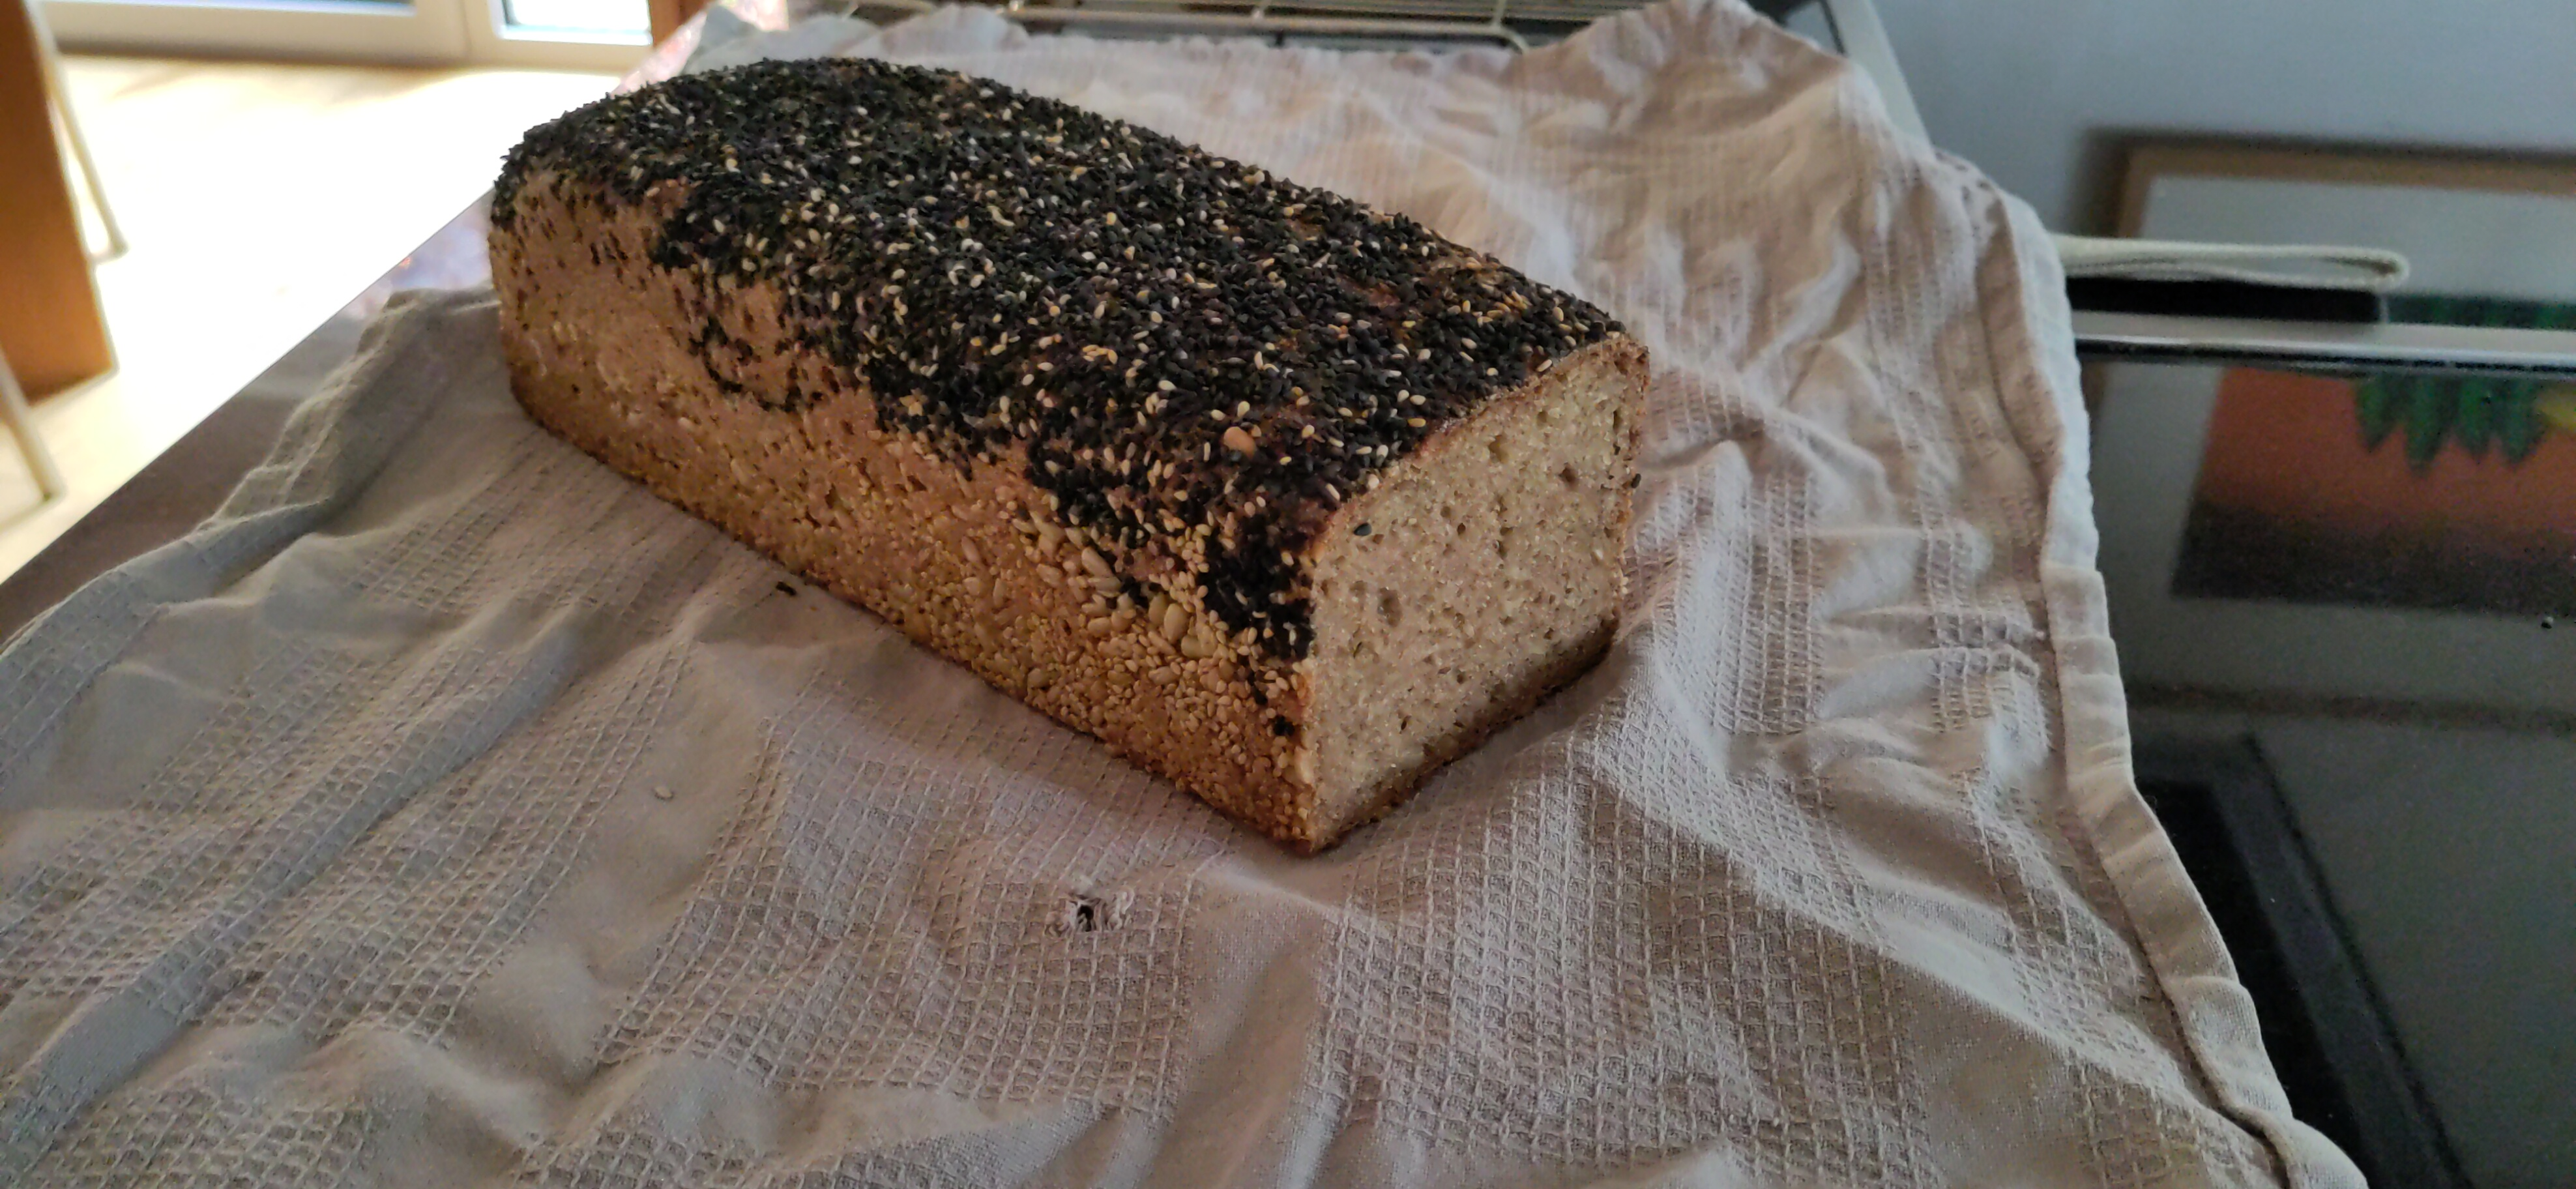
\includegraphics[width=0.7\linewidth]{Bilder/Vollkornprotz}
%%    \caption{Vollkornprotz mit schwarzem Sesam}
%%    \label{fig:vollkornprotz}
%\end{figure}

\subsection*{Zeitplan}
\begin{tabular}{ r @{ Uhr \phantom{bla} } l}
    \toprule
    \multicolumn{1}{c @{\phantom{ bla }}}{Zeit} & \multicolumn{1}{@{}l}{Aktion}      \\ \midrule
    00:00                                       & \Gls{Sauerteig} schnell  / langsam \\
    03:00 / 11:00                               & \Gls{Autolyse}                     \\
    04:00 / 12:00                               & \Gls{Hauptteig}                    \\
    04:20 / 12:20                               & \Gls{Stockgare}                    \\
    06:20 / 14:20                               & Formen + \Gls{Stueckgare}          \\
    07:50 / 15:50                               & Backen                             \\
    08:40 / 16:40                               & fertig                             \\ \bottomrule
\end{tabular}
%
\subsection*{Zutaten}
\begin{tabular}{r l}
    50\;g / 7\;g g & Roggen ASG               \\
             25\;g & Roggen Vollkorn          \\
            200\;g & Roggen 1150              \\
            150\;g & Malzbier                 \\
             60\;g & Weizen Tipo 00           \\
             60\;g & Weizen 550               \\
            130\;g & Weizen 1050              \\
              30 g & Zucker                   \\
             12\;g & Salz                 \\
             2\; g & Frischhefe               \\
\end{tabular}\\

\subsection*{Zubereitung}
\begin{enumerate}
    \item [\Gls{Sauerteig}] Mild im Aroma\\ \textbf{Zutaten:}\\
    \begin{tabular}{r l}
        50\;g & Roggen ASG      \\
        25\;g & Roggen Vollkorn \\
        25\;g & Roggen 1150     \\
        40\;g & Wasser
    \end{tabular}

    Alle Zutaten gründlich mischen. Für 2–4 Stunden bei 26--28°\;C reifen lassen.
    
    \item [\Gls{Sauerteig}] Kräftig im Aroma\\ \textbf{Zutaten:}\\
    \begin{tabular}{r l}
        6\;g & Roggen ASG      \\
        35\;g & Roggen Vollkorn \\
        40\;g & Roggen 1150     \\
        75\;g & Wasser
    \end{tabular}

    Alle Zutaten gründlich mischen. Für 10--12 Stunden bei 22°\;C reifen lassen.

    \item [\Gls{Autolyse}]  \textbf{Zutaten:}\\
    \begin{tabular}{r l}
        160\;g & Wasser 30°\;C  \\
        150\;g & Malzbier       \\
         60\;g & Weizen Tipo 00 \\
         60\;g & Weizen 550     \\
        130\;g & Weizen 1050
    \end{tabular}

    Alles kurz, aber gründlich mischen. Für 60 Minuten abgedeckt quellen lassen.

    \item [\Gls{Hauptteig}]  \textbf{Zutaten:}\\
    \begin{tabular}{r l}
        + & Autolyse  \\
        + & Sauerteig       \\
        2\;g & Hefe \\
        13\;g & Roggen 1150     \\
        12\;g & Salz
    \end{tabular}

    Alle Zutaten des Hauptteigs für 5--8 Minuten bei langsamer Geschwindigkeit mischen. 

    \item [\Gls{Stockgare}] Abgedeckt 90–120 Minuten bei 25–27° C zur Gare stellen.

    \item [\Gls{Formen}] Auf der bemehlten Arbeitsfläche rund wirken. Mit dem Schluss nach unten in ein bemehltes Gärkörbchen geben.
    \item[\Gls{Stueckgare}] Abgedeckt für 90 Minuten bei Raumtemperatur zur Gare stellen.
    \item[\Gls{Backen}] 250° C Ober–/Unterhitze vorheizen.\\
    Teigling aus dem Gärkörbchen stürzen und einschießen. Sofort schwaden und für insgesamt 50 Minuten backen. Nach 10 Minuten den Dampf ablassen und die Temperatur auf 210° C reduzieren.
\end{enumerate}

\section[Rosinenbrot]{Rosinenbrot \textmd{(siehe \cite{sonjarosinenbrot2023})} }  \index{Brot!Rosinen}\index{Brot!Weizen 550}\index{Brot!Lievito Madre}
\subsection*{Zeitplan}
\begin{tabular}{ r @{ Uhr \phantom{bla} } l}
    \toprule
    \multicolumn{1}{c @{\phantom{ bla }}}{Zeit} & \multicolumn{1}{@{}l}{Aktion}         \\ \midrule
    00:00                                       & \Gls{Quellstueck} \Gls{Auffrischen}  \\
    04:00                                       & \Gls{Hauptteig}                       \\
    04:20                                       & \Gls{Stockgare}                       \\
    08:20                                       & Formen und \Gls{Zwischengare}         \\
    09:00                                       & \Gls{Stueckgare} Kühlschrank          \\
    20:00                                       & Akklimatisieren                       \\
    20:10                                       & Backen                                \\
    20:50                                       & fertig                                \\ \bottomrule
\end{tabular}


%\begin{figure}[H]
%%    \centering
%%    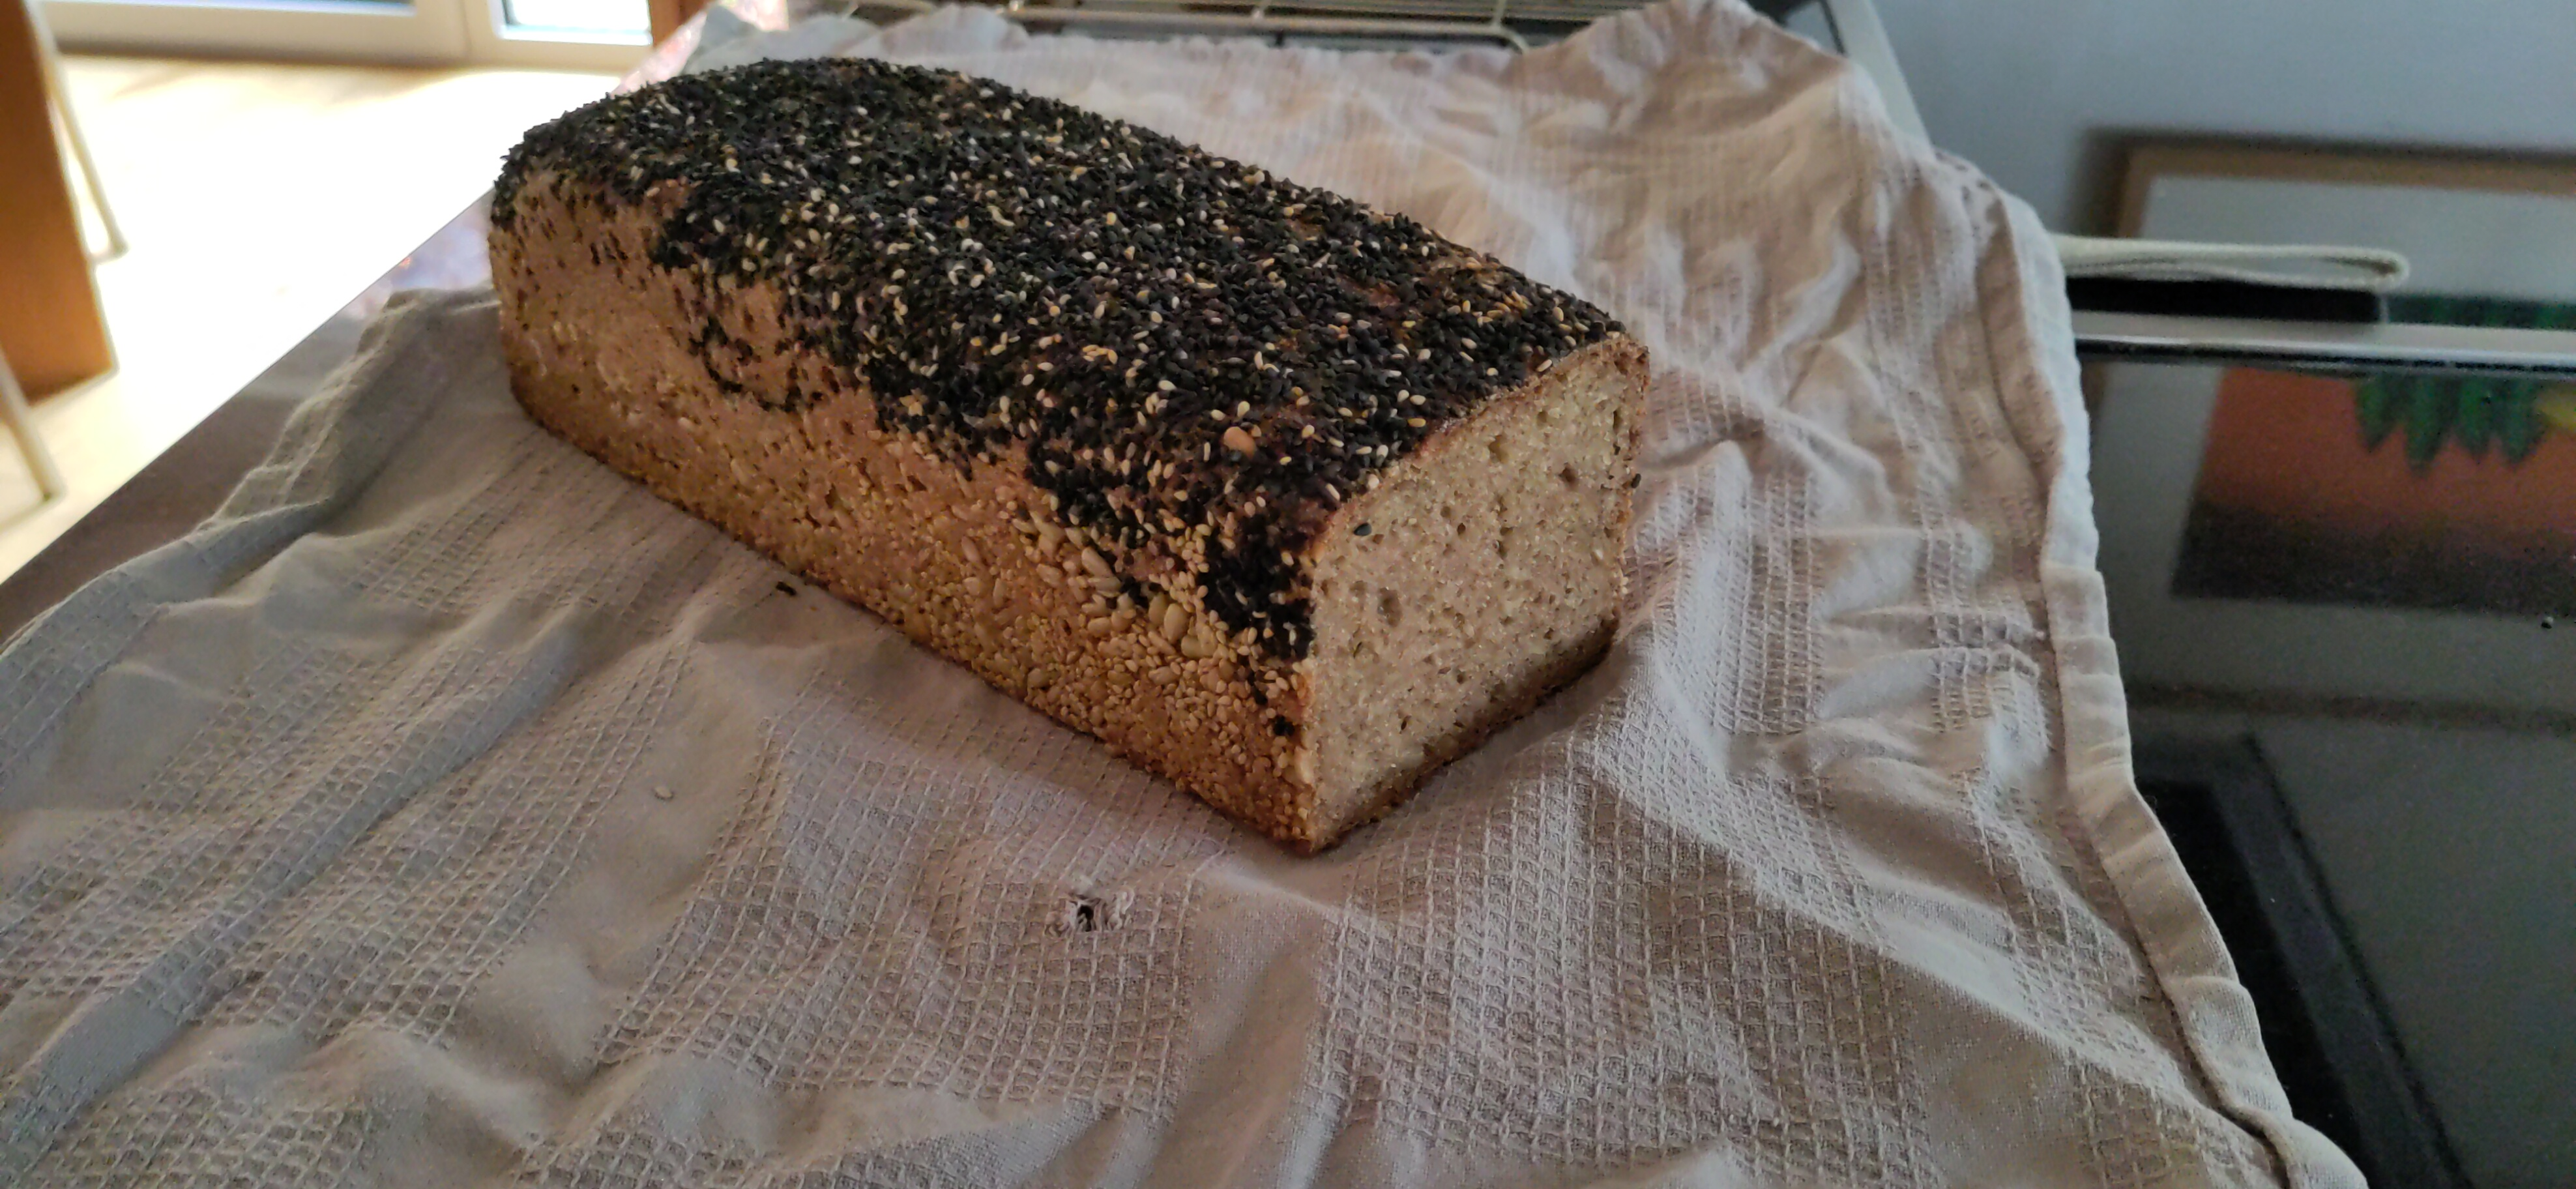
\includegraphics[width=0.7\linewidth]{Bilder/Vollkornprotz}
%%    \caption{Vollkornprotz mit schwarzem Sesam}
%%    \label{fig:vollkornprotz}
%\end{figure}
%
%
\subsection*{Zutaten}
\begin{tabular}{r l}
          475 g & Weizenmehl Type 550          \\
          320 g & Milch (ca. 3,5\% Fett)       \\
          120 g & Rosinen                      \\
           75 g & aufgefrischter \Gls{LievitoMadre} \\
           60 g & Butter                       \\
           60 g & Milch                        \\
           30 g & Zucker Vanillezucker         \\
           30 g & Zucker                       \\
            8 g & Salz                         \\
            5 g & Frischhefe                   \\
              2 & Ei(er), Gr. M                \\
    0.5 Zitrone & Abrieb Versuch weglassen
\end{tabular}\\



\subsection*{Zubereitung}
\begin{enumerate}
    \item [\Gls{Auffrischen}] \textbf{Zutaten:}\\
         Für aufgefrischten Lievito Madre siehe \vref{sec:Lievito Madre},
    
    \item [\Gls{Quellstueck}] \textbf{Zutaten:}\\
        \begin{tabular}{r l}
            120 g  & Rosinen  \\
            60 g &  Milch  
        \end{tabular}
        
        Die Rosinen mit der Milch (ggf, 20 g durch Rum ersetzen) mischen und abgedeckt mindestens 4 Stunden oder über Nacht (im Kühlschrank) einweichen.
    \item  [\Gls{Hauptteig}] \textbf{Zutaten:}\\
        \begin{tabular}{r l}
            475 g & Weizenmehl Type 550                   \\
            260 g & Milch (ca. 3,5\% Fett)                \\
            75 g & aufgefrischter Lievito Madre          \\
            60 g & Butter                                \\
            30 g & Zucker Vanillezucker                  \\
            30 g & Zucker                                \\
            8 g & Salz                                  \\
            5 g & Frischhefe                            \\
            1 & Ei(er), Gr. M                         \\
            0.5 Zitrone & Abrieb Versuch weglassen              \\
            & Quellstück (abgetropft)               \\
            & abgetropfte Flüssigkeit als Bassinage
        \end{tabular}
        
        Alle Zutaten für den Teig (außer Butter und Salz) etwa 10 Minuten bei langsamer Geschwindigkeit in der Küchenmaschine kneten.\\
        Anschließend etwa 5–8 Minuten bei höherer Geschwindigkeit weiter kneten, dabei portionsweise die Butter und das Salz hinzufügen. Dabei nach Bedarf noch bis zu 20 g der Flüssigkeit des Quellstücks mit einkneten.\\
        Zum Schluss das abgetropfte Quellstück kurz mit der Hand oder bei langsamer Geschwindigkeit mit der Küchenmaschine unter den Teig kneten.
    \item  [\Gls{Stockgare}] Den Teig in einer leicht geölten Schüssel oder Teigwanne abgedeckt bei
    Raumtemperatur etwa 3 bis 4 Stunden bis zur guten Verdopplung reifen lassen.\\
    Dabei nach 1 Stunde dehnen und falten.
    \item [\GLS{Formen}] Eine 1-kg-Brotbackform (23 × 11 × 9,5 cm) einfetten und leicht bemehlen.\\
     Den Teig auf der leicht bemehlten Arbeitsfläche (z. B. mit Weizendunst) länglich formen und in die vorbereitete Kastenform geben.
    \item [\Gls{Stueckgare}] Abgedeckt 30–40 Minuten bei Raumtemperatur anspringen lassen, danach für etwa 10–12 Stunden im Kühlschrank bei 5 °C weiter reifen lassen.
    \item [Backen] \textbf{Zutaten:}\\
    \begin{tabular}{r l}
        1 & Ei     \\
        10g & Milch  \\
        1 Prise & Zucker \\
        1 Prise & Salz
    \end{tabular}
    
    Den Backofen rechtzeitig auf 210 °C Ober-/Unterhitze vorheizen.\\
    Für die Eistreiche alle Zutaten gründlich miteinander verquirlen und danach gerne durch ein Sieb streichen. \\
    Die Kastenform aus dem Kühlschrank nehmen und den Teig mit der Eistreiche bestreichen. \\
    Danach einmal längs einschneiden und in den vorgeheizten Backofen einschießen und insgesamt etwa 40–45 Minuten backen. Je nach Backform und
    Backofen kann die sich die Backzeit etwas verlängern, auf 50 bis max. 60 Minuten; Die Kerntemperatur sollte 90–93 °C erreichen.\\
    Dabei nach 1–2 Minuten Backzeit verzögert schwaden und die Temperatur auf 180 °C Ober-/Unterhitze  reduzieren.\\
    Den Schwaden während der gesamten Backzeit nicht ablassen. \\
    Nach dem Backen aus der Kastenform nehmen, mit einem leicht feuchtem Geschirrtuch bedeckt auf einem Rost auskühlen lassen. 
\end{enumerate}



\section{Mohnkruste}  \index{Brot!Mohn}\index{Brot!Weizen}\index{Brot!Lievito Madre}

%%\begin{figure}[H]
%%%    \centering
%%%    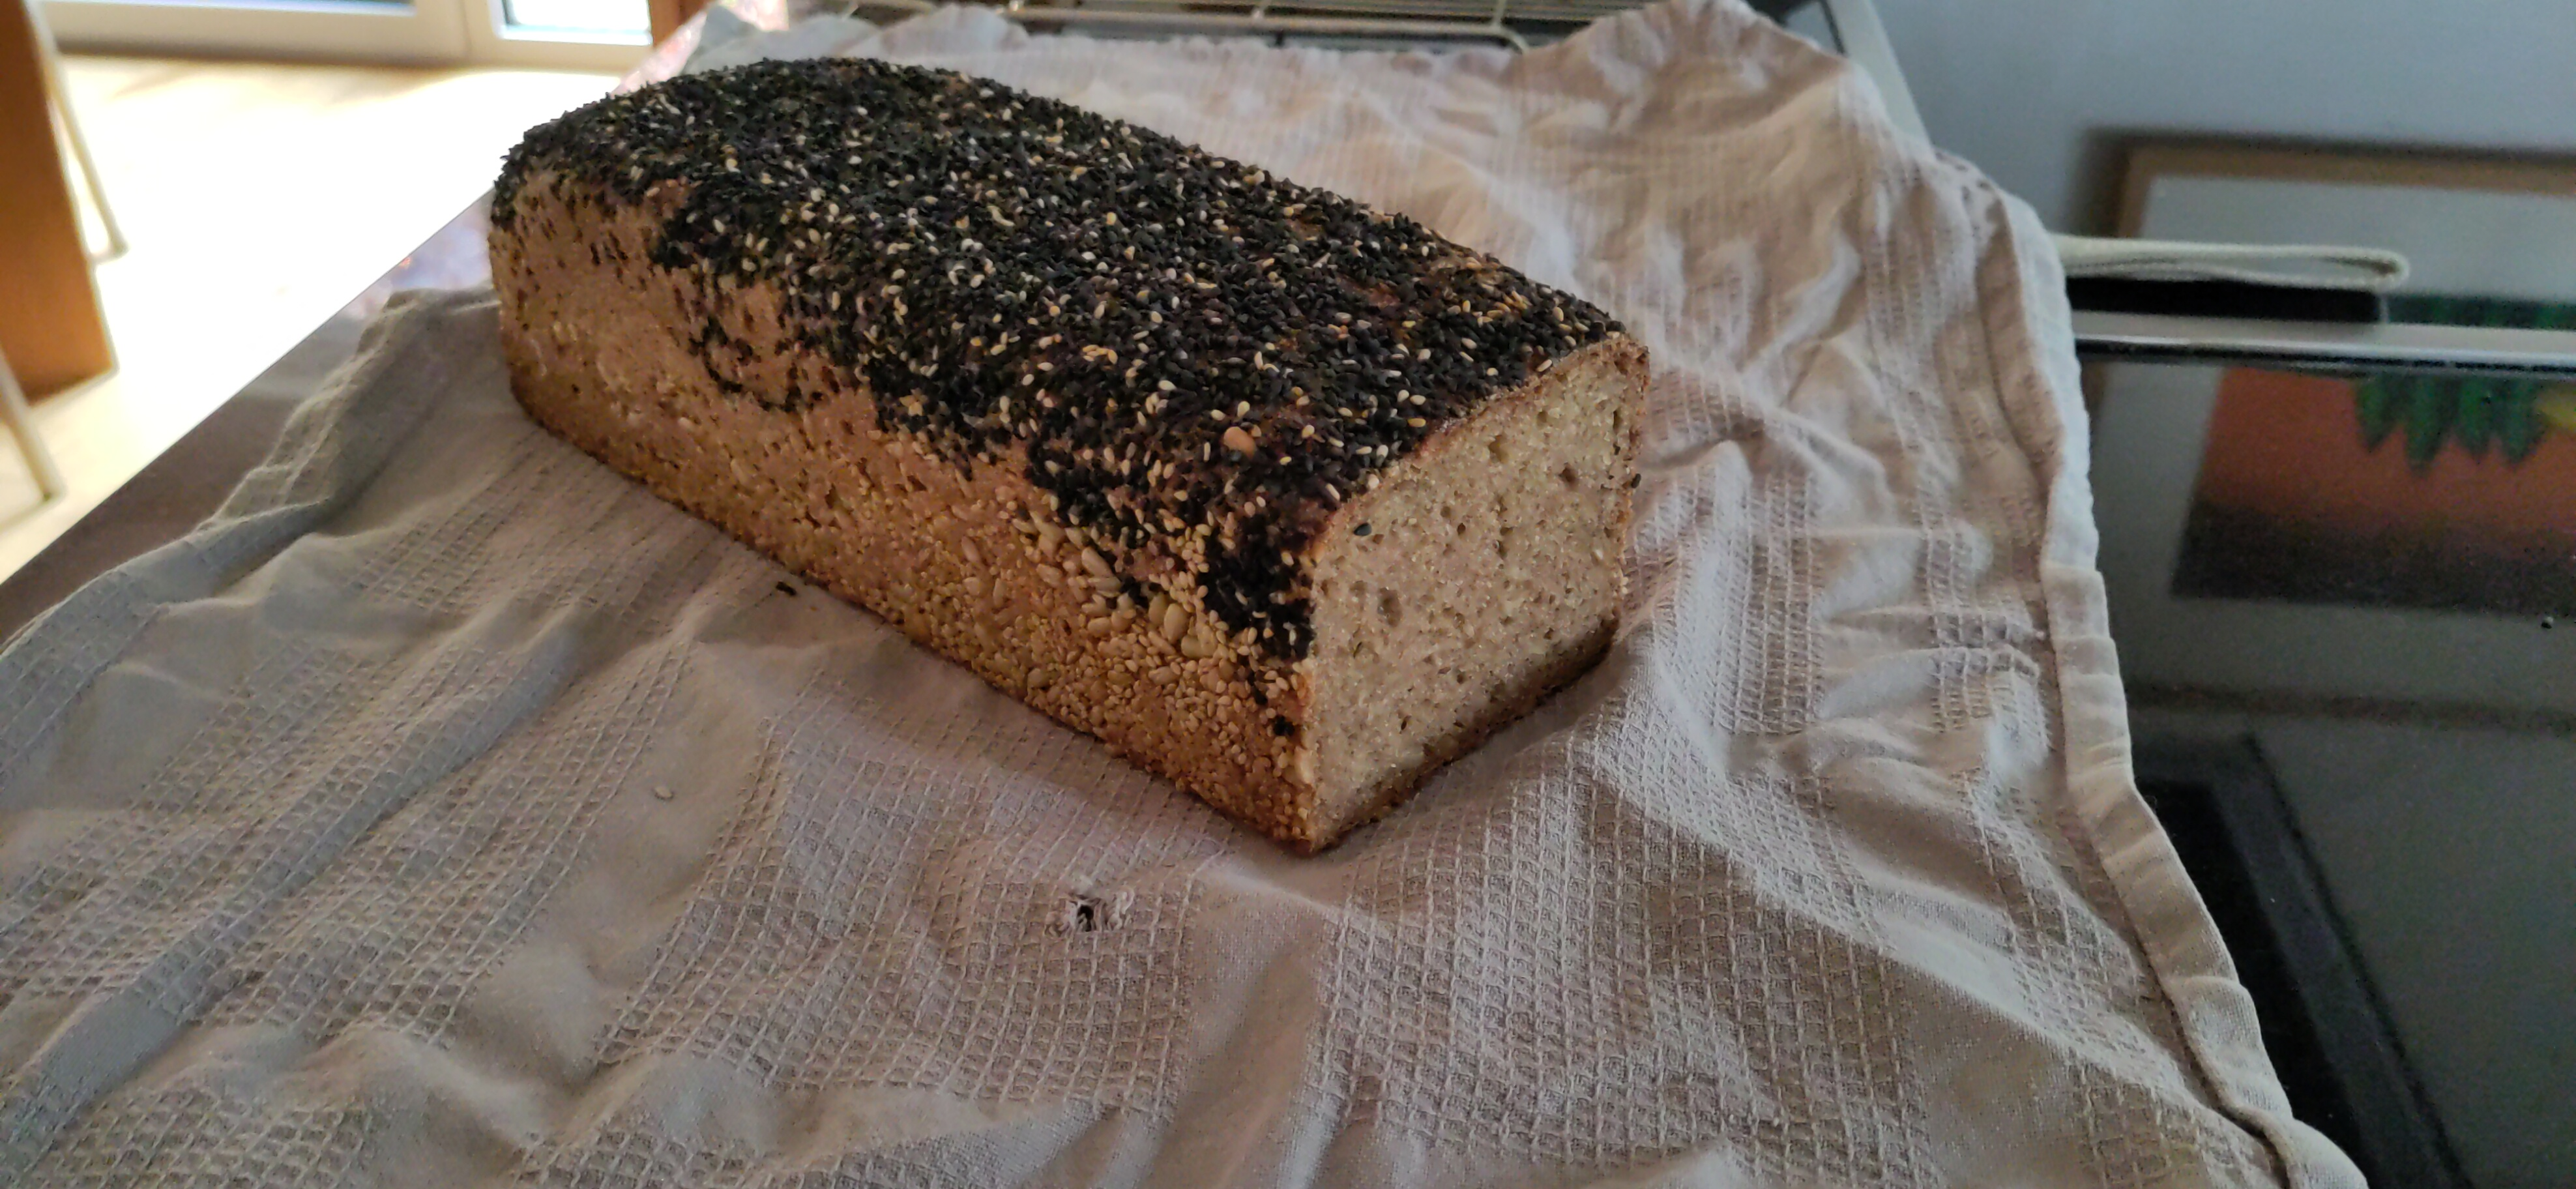
\includegraphics[width=0.7\linewidth]{Bilder/Vollkornprotz}
%%%    \caption{Vollkornprotz mit schwarzem Sesam}
%%%    \label{fig:vollkornprotz}
%%\end{figure}
%%
%%
%%\subsection*{Hauptteig}
%A U T O LY S E
%350 g
%350 g
%100 g
%50 g
%Wasser, kühl
%Weizenmehl T 550
%Weizenmehl T 1050
%Weizenvollkornmehl
%HAUP T TEIG
%+
%1 g
%10 g
%12 g
%30 g
%± 30 g
%Autolyse
%Frischhefe
%Honig
%Salz
%Mohn
%Wasser bei Bedarf
%(Bassinage)
%ZU S ÄT ZL I C H
%Mohn
%
%%
%%\subsection*{Zubereitung}
%Kurz, aber gründlich vermischen.
%Für 30 Minuten abgedeckt quellen lassen.
%M E N G E : ca . 9 2 0 g •
%TE I GTE M P E R A TU R : 24–26° C
%Alle Zutaten (außer Salz + Bassinage) für 8–10 Minuten mit
%geringer Stufe kneten. Salz zugeben, für 3–5 Minuten
%mit höherer Stufe auskneten und bei Bedarf portions-
%weise bis zu 30 g Wasser (Bassinage) mit einkneten.
%Ohne Hefe:
%Statt 1 g Hefe können auch 40 g Lievito Madre
%(LM, aufgefrischt) ver wendet werden.
%Für 10–12 Stunden bei 22–24° C zur Stockgare stellen.
%
%M O HNK RUS T E
%Einfaches Weizenbrot mit Mohn
%1 0 –1 2 S T D.
%2 0 –2 2° C
%D + F:
%4 5 | 90 MIN.
%S T O C KG A R E
%Z I E L : etwa Verdopplung
%Abgedeckt für 10–12 Stunden bei Raumtemperatur zur Gare stellen.
%Nach 45 und 90 Minuten dehnen und falten (D + F) .
%FORMEN
%Auf der bemehlten Arbeitsfläche schonend rund wirken und mit
%dem Schluss nach oben in ein bemehltes Gärkörbchen geben.
%6 0 –9 0 M IN .
%2 0 –2 2° C
%ODER
%1 2–1 4 S T D.
%5 – 6° C
%S T Ü C KG A R E
%Z I E L : k n a p p e G a r e (siehe S. 69)
%Abgedeckt für 60–90 Minuten bei Raumtemperatur zur Gare stellen.
%O D E R : Ohne Anspringen für 12–14 Stunden bei 5–6° C im Kühlschrank zur
%Gare stellen. Anschließend ohne Akklimatisieren backen.
%5 0 M IN .
%2 5 0° C
%2 1 0° C
%BACKEN
%Backofen rechtzeitig mit einem Backstahl, Backstein oder Gusstopf auf
%250° C Ober–/Unterhitze vorheizen.



\section[Quarkstuten]{Quarkstuten \textmd{(siehe \cite[296]{SonjaBauer2021})} }  \index{Brot!Quark}\index{Brot!Weizen}\index{Brot!Lievito Madre}
\subsection*{Zeitplan}
\begin{tabular}{ r @{ Uhr \phantom{bla} } l}
    \toprule
    \multicolumn{1}{c @{\phantom{ bla }}}{Zeit} & \multicolumn{1}{@{}l}{Aktion}   \\ \midrule
    -03:30                                      & \Gls{LievitoMadre}              \\
    00:00                                       & \Gls{Hauptteig}                 \\
    00:20                                       & \Gls{Stockgare}                 \\ \midrule
    03:50                                       & Formen und \Gls{Zwischengare}   \\
    04:05                                       & \Gls{Stueckgare} Raumtemperatur \\
    05:50                                       & Backen                          \\
    06:30                                       & fertig                          \\ \midrule
    04:05                                       & \Gls{Stueckgare} Kühlschrank    \\
    15:05                                       & Akklimatisieren                 \\
    15:35                                       & Backen                          \\
    16:15                                       & fertig                          \\ \bottomrule
\end{tabular}

%L I E V I T O M A D R E (LM)
%15 g
%30 g
%30 g
%Wasser, 40° C
%LM
%Weizenmehl T 550
%Z I E L : mindestens Verdopplung
%Lievito Madre mit dem Wasser schaumig aufschlagen.
%Danach mit dem Mehl verkneten. Für 2–4 Stunden bei
%26–30° C reifen lassen.
%HAUP T TEIG
%150 g
%100 g
%+
%5 g
%1
%1
%60 g
%1
%10 g
%500 g
%60 g
%5 g
%± 30 g
%Quark/Topfen, kalt
%Milch, kalt
%LM
%Frischhefe
%Ei (Gr. M) , kalt
%Eiklar, kalt
%Zucker
%unbehandelte Zitrone,
%davon den Schalenabrieb
%Bourbon-Vanillezucker
%Weizenmehl T 550
%Butter, kühl
%Salz
%Milch bei Bedarf
%( Bassinage)
%M E N G E : ca. 1 .0 8 0 g • TE I GTE M P E R A TU R : 2 4 –2 6° C
%Alle Zutaten (außer Butter + Salz + Bassinage) für 10 Mi-
%nuten bei geringer Stufe kneten. Für 5–8 Minuten bei
%höherer Stufe auskneten. Dabei Salz, portionsweise
%die Butter und bei Bedarf noch bis zu 30 g Milch
%(Bassinage) mit einkneten.
%Hinweis:
%Statt Lievito Madre können insgesamt 10 g
%Frischhefe + 50 g Mehl + 25 g Wasser an den
%Hauptteig gegeben werden.
%EISTREICHE
%1
%10 g
%1 Prise
%Eigelb (das übrig gebliebene)
%Milch/Sahne
%Salz + Zucker
%Alle Zutaten kurz verquirlen und bereitstellen.
%ZU S ÄT ZL I C H : Hagelzucker und gehobelte Mandeln

%S T O C KG A R E
%Z I E L : et wa Verdopplung
%Abgedeckt für etwa 3–4 Stunden bei Raumtemperatur zur Gare stellen.
%Nach 60 Minuten dehnen und falten (D + F).
%FORMEN + ZWISCHENGARE
%Kastenform einfetten und leicht bemehlen oder mit Backpapier/Dauerbackfolie auslegen.
%Anschließend den Teig in 2 Teile à ca. 540 g teilen.
%Diese jeweils locker rund wirken und abgedeckt für 10 Minuten ruhen lassen (Zwischengare).
%Danach zu 2 Strängen von etwa 40 cm formen, diese kordelartig ineinander verschlingen
%und in die vorbereitete Backform legen.
%Mit der Eistreiche bestreichen, die restliche Eistreiche kaltstellen.
%S T Ü C KG A R E
%Z I E L : 2– 3 c m ü b e r d e n R a n d d e r F o r m
%Abgedeckt für etwa 90–120 Minuten bei Raumtemperatur zur Gare stellen. Der Teig
%sollte deutlich aufgegangen sein, beziehungsweise im Idealfall 2–3 cm über den Rand
%der Kastenform reichen.
%O D E R : Abgedeckt für 30 Minuten anspringen lassen, danach für etwa 10–12 Stunden
%im Kühlschrank bei 5° C zur Gare stellen. Anschließend für 30–60 Minuten bei Raum-
%temperatur akklimatisieren lassen.
%BACKEN
%Backofen rechtzeitig auf 210° C Ober-/Unterhitze vorheizen.
%Den Teigling erneut mit der Eistreiche einstreichen und mit Hagelzucker und gehobelten
%Mandeln bestreuen. Einschießen und die Temperatur auf 180° C reduzieren.
%Für insgesamt etwa 40 Minuten backen. Bei zu starker Bräunung rechtzeitig abdecken.

\chapter{Auffrischbrote}

\section[Frühstücksbrot]{Frühstücksbrot \textmd{(siehe \cite[227]{SonjaBauer2021})} }  \index{Auffrischbrot!Frühstücksbrot}\index{Brot!Auffrischbrot}\index{Brot!Weizen}\index{Brot!Lievito Madre}

\subsection*{Zeitplan}
\begin{tabular}{ r @{ Uhr \phantom{bla} } l}
    \toprule
    \multicolumn{1}{c @{\phantom{ bla }}}{Zeit} & \multicolumn{1}{@{}l}{Aktion} \\ \midrule
    00:00                                       & \Gls{Hauptteig}               \\
    00:20                                       & \Gls{Stockgare}               \\
    03:50                                       & Formen und \Gls{Zwischengare} \\
    04:35                                       & \Gls{Stueckgare} Kühlschrank  \\
    15:35                                       & Akklimatisieren               \\
    15:50                                       & Backen                        \\
    16:30                                       & fertig                        \\ \bottomrule
\end{tabular}
%
\subsection*{Zutaten}
%\subsubsection*{Alle Zutaten}
\begin{tabular}{r l}
    150 g & Wasser, kühl         \\
    150 g & Milch, kalt     \\
    75g & Lievito Madre \\
    2 g & Frischhefe            \\
    450 g & Weizenmehl T 550     \\
    10 g & Honig            \\
    20 g & Butter kühl \\
    11 g & Salz                  \\
    Zusätzlich & Mohn oder Sesam
\end{tabular}\\

\subsection*{Zubereitung}
\begin{enumerate}
    \item  [\Gls{Hauptteig}]  Alle Zutaten (außer Butter + Salz + Bassinage) für 10 Minuten bei geringer Stufe kneten. Salz und Butter hinzufügen, für 5–8 Minuten bei höherer Stufe auskneten und bei Bedarf portionsweise bis zu 25 g     Wasser (Bassinage) mit einkneten.
    \item [\Gls{Stockgare}] Abgedeckt für 3–4 Stunden bei Raumtemperatur zur Gare stellen. Nach 60 und 120 Minuten dehnen und falten (D + F) . 
    \item [\Gls{Formen}] Den Teig auf der leicht bemehlten Arbeitsfläche zu zwei runden Teiglingen je ca. 450 g formen. Mit dem Schluss nach unten in eine gefettete Kastenform geben. Teiglinge anfeuchten und mit Mohn oder Sesam bestreuen.
    \item [\Gls{Stueckgare}] Abgedeckt 30–40 Minuten bei Raumtemperatur anspringen lassen, danach für etwa 10–12 Stunden im Kühlschrank bei 5 °C weiter reifen lassen.
    \item [\Gls{Backen}] Kastenform aus dem Kühlschrank nehmen. Backofen rechtzeitig mit einem Backstahl 230° C Ober-/Unterhitze vorheizen.Teigling längs einschneiden und einschießen. Sofort schwaden und die Temperatur auf 200° C reduzieren.\\ 
    Für insgesamt 40 Minuten backen. Nach 10 Minuten den Dampf ablassen. Nach dem Backen sofort mit etwas Wasser einsprühen.   
\end{enumerate}



\section{Auffrischbrötchen Julchen}  \index{Brot!Weizen}\index{Brot!Lievito Madre}\index{Auffrischbrot! Brötchen Julchen}
\cite{sonjajulchen2022}
\subsection*{Zeitplan}
\begin{tabular}{ r @{ Uhr \phantom{bla} } l}
    \toprule
    \multicolumn{1}{c @{\phantom{ bla }}}{Zeit} & \multicolumn{1}{@{}l}{Aktion} \\ \midrule
    00:00                                       & \Gls{Fermentolyse}            \\
    00:30                                       & \Gls{Hauptteig}               \\
    00:50                                       & \Gls{Stockgare}               \\
    01:50                                       & \Gls{DehnenUndFalten}         \\
    02:50                                       & \Gls{DehnenUndFalten}         \\
    03:50                                       & \Gls{Formen}                  \\
    04:00                                       & \Gls{Stueckgare}              \\
    04:30                                       & \GLS{Vorheizen}               \\
    05:00                                       & \GLS{Backen}                  \\
    05:20                                       & fertig                        \\ \bottomrule
\end{tabular}


\subsection*{Zutaten}
\subsubsection*{Fermentolyseteig}
\begin{tabular}{r l}
    75 g & Lievito-Madre-Anstellgut\\
    180 g & kalte Vollmilch (oder pflanzliche Alternative)\\
    145 g & kühles Wasser\\
    400 g & Weizenmehl Type 550\\
    50 g & Vollkornmehl nach Wahl\\
\end{tabular}\\
Alles kurz, aber gründlich mischen und für 20−30 Minuten abgedeckt quellen lassen.


\subsubsection*{Hauptteig}
\begin{tabular}{r l}
    & Fermentolyseteig                                      \\
    5 g & Frischhefe (oder 3 g bei kalter Übernachtgare         \\
    10 g & Honig  \\
    11 g & Salz                                                  \\
    10 g & Butter (oder Olivenöl)                                \\
    20 g & Wasser nach Bedarf (Bassinage)                        \\
    & Roggenmehl zum Aufarbeiten (z. B. Type 610 oder 1150)
\end{tabular}\\


\subsection*{Zubereitung}
\begin{enumerate}
    \item [Teig] 
    \begin{itemize}
        \item Die Frischhefe und den Blütenhonig zum Fermentolyseteig geben und für 10 Minuten mit geringer Stufe kneten.
        \item Danach das Salz und die Butter zugeben und für 3–5 Minuten mit höherer Stufe auskneten, dabei bei Bedarf noch bis zu 20 g Wasser mit einkneten. )]
    \end{itemize}
    \item [Stockgare]
    \begin{itemize}
        \item Den Teig in einer leicht geölten Schüssel oder Teigwanne bei Raumtemperatur abgedeckt etwa 3 Stunden bis zur guten Verdopplung reifen lassen, dabei nach 1 und 2 Stunden schonend dehnen und falten (Coil fold).
        \item Variation kalte Stockgare: Für 90 Minuten bei Raumtemperatur (20−22 °C) anspringen lassen. Dabei nach jeweils 45 und 90 Minuten dehnen und falten. Danach für 12−14 Stunden bei 5 °C in den Kühlschrank geben. Anschließend für mindestens 1 Stunde akklimatisieren lassen.
    \end{itemize}
    \item [Formen]
    \begin{itemize}
        \item Den Teig auf der bemehlten Arbeitsfläche in neun Teile mit je etwa 95 g teilen.
        \item Die Teiglinge schonend rund wirken und dabei Roggenmehl in den Teigschluss einarbeiten, damit dieser während der Stückgare nicht verklebt.
        \item Danach mit dem Teigschluss nach unten in ein leicht bemehltes Bäckerleinen oder Geschirrtuch legen und den Stoff zwischen den Teiglingen etwas hochziehen, damit diese gestützt werden.
    \end{itemize}
    \item [\Gls{Stueckgare}]
    \begin{itemize}
        \item Die Teiglinge abgedeckt bei Raumtemperatur (20−22 °C) etwa 60–80 Minuten bis zur knappen Gare reifen lassen.
        \item Variation kalte Stückgare:  Die Teiglinge ohne Anspringen (gut eingepackt, z. B. mit XXL Gefrierbeuteln*) über Nacht 10–12 Stunden in den Kühlschrank bei 4–5 °C reifen lassen. (Die Kühlschranktemperatur bitte unbedingt nachmessen!) Danach ohne Akklimatisieren backen.
    \end{itemize}
    \item [Backen]
    \begin{itemize}
        \item Den Backofen rechtzeitig auf 240 °C Ober-/Unterhitze (220 °C Heißluft/Umluft) vorheizen, zusammen mit einem Backstahl oder Backstein.
        \item Die Teiglinge mit dem Teigschluss nach oben auf einem Bogen Backpapier oder Dauerbackfolie auf dem Einschießer verteilen.
        \item Anschließend einschießen und sofort schwaden. Insgesamt etwa 18−20 Minuten backen. Nach 10 Minuten den Dampf ablassen und die Temperatur auf 200 °C (180 °C Heißluft/Umluft) reduzieren.
        \item Anschließend sofort mit etwas Wasser einsprühen und auf einem Rost auskühlen lassen.
    \end{itemize}
\end{enumerate}

\section[Mediterranes Landbrot]{Mediterranes Landbrot  \textmd{(siehe \cite{sonjaMedLandbrot2019})} }  \index{Auffrischbrot!Mediterranes Landbrot}\index{Brot!Auffrischbrot}\index{Brot!Weizen}\index{Brot!Lievito Madre}

\subsection*{Zeitplan}
\begin{tabular}{ r @{ Uhr \phantom{bla} } l}
    \toprule
    \multicolumn{1}{c @{\phantom{ bla }}}{Zeit} & \multicolumn{1}{@{}l}{Aktion}       \\ \midrule
    00:00                                       & Lievito Madre im Wasser aufschlagen \\
    00:35                                       & \Gls{Fermentolyse}                  \\
    01:35                                       & \Gls{Hauptteig}                     \\
    01:50                                       & \Gls{Stockgare}                     \\
    05:20                                       & Formen und                          \\
    05:30                                       & \Gls{Stueckgare} Kühlschrank        \\
    14:00                                       & \GLS{Vorheizen}                     \\
    14:30                                       & \GLS{Backen}n                       \\
    15:45                                       & fertig                              \\ \bottomrule
\end{tabular}
%
\subsection*{Zutaten}
%\subsubsection*{Alle Zutaten}
\begin{tabular}{r l}
    340 g & Wasser, kühl         \\
    200g & Lievito Madre \\
    200 g & Semola  \\
    200 g & Tipo 0 ersatzweise Tippo 00 oder 550 \\
    1 g & Hefe     \\
    10 g & Honig            \\
    15 g & Olivenöl \\
    11 g & Salz                  
\end{tabular}\\

\subsection*{Zubereitung}
\begin{enumerate}
    \item [Lievito Madre] in dem Wasser sehr schaumig aufschlagen.
    \item [\GLS{Fermentolyse}] Mehl hinzufügen und kurz untermischen und 60 Minuten quellen lassen
    
    \item  [\Gls{Hauptteig}]  Alle Zutaten (außer Butter + Salz) für 10 Minuten bei geringer Stufe kneten. Salz und Öl hinzufügen, für 5 Minuten bei höherer Stufe auskneten.
    \item [\Gls{Stockgare}] Abgedeckt für 3–4 Stunden bei Raumtemperatur zur Gare stellen. Nach 30 und 60 Minuten dehnen und falten (D + F) . 
    \item [\Gls{Formen}] Den Teig auf der leicht bemehlten Arbeitsfläche zu einem Brotlaib formen. Mit dem Schluss nach oben in ein mit Semola bemehltes Gärkörbchen geben.
    \item [\Gls{Stueckgare}]  Für etwa 8-10 Stunden im Kühlschrank bei 8 °C weiter reifen lassen.
    \item [\Gls{Backen}] Backofen rechtzeitig auf 250° C Ober–/Unterhitze vorheizen.\\
    Teigling aus dem Gärkörbchen stürzen und einschießen. Sofort schwaden und für insgesamt 45
    Minuten backen. Nach 10 Minuten den Dampf ablassen und die Temperatur auf 210° C reduzieren.
\end{enumerate}


\section[Jules Schwester]{Jules Schwester \textmd{(siehe \cite[112]{SonjaBauer2021})}}  \index{Brot!Weizen}\index{Brot!Lievito Madre}\index{Auffrischbrot! Jules Schwester}

\begin{figure}[H]
    \centering
    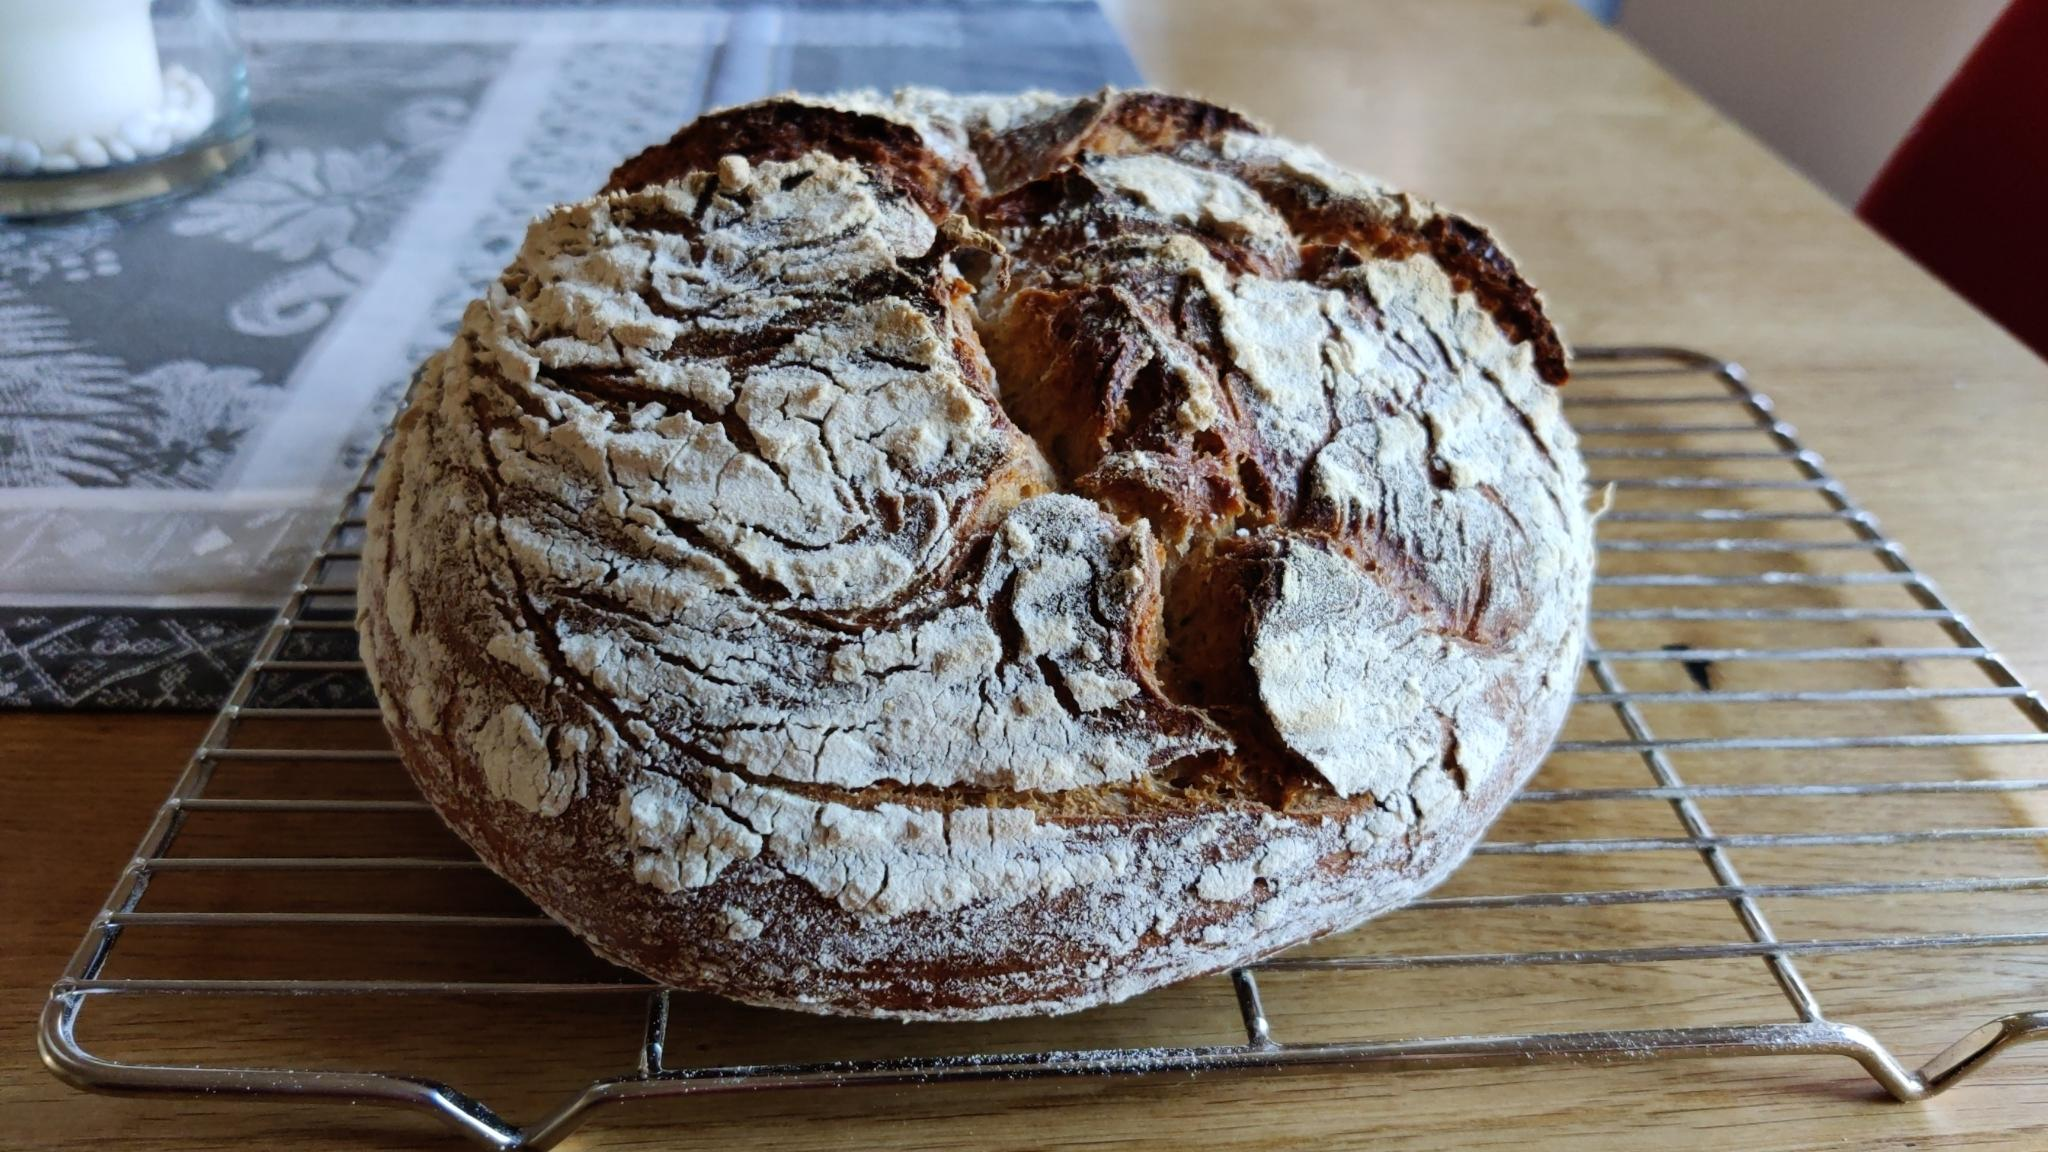
\includegraphics[width=0.7\linewidth]{Bilder/JulesSchwester}
    \caption{Jules Schwester}
    \label{fig:auffrischbrotJulesSchwester}
\end{figure}

\subsection*{Zeitplan}
\begin{tabular}{ r @{ Uhr \phantom{bla} } l}
    \toprule
    \multicolumn{1}{c @{\phantom{ bla }}}{Zeit} & \multicolumn{1}{@{}l}{Aktion} \\ \midrule
    00:00                                       & \Gls{Bruehstueck}             \\
    00:20                                       & \Gls{Fermentolyse}            \\
    01:00                                       & \Gls{Hauptteig}               \\
    01:20                                       & \Gls{Stockgare}               \\
    02:20                                       & \Gls{DehnenUndFalten}         \\
    03:50                                       & \Gls{Formen}                  \\
    04:00                                       & \Gls{Stueckgare}              \\
    05:30                                       & \Gls{Backen}                  \\
    07:10                                       & fertig                        \\ \bottomrule
\end{tabular}
%
%
\subsection*{Alle Zutaten}
\begin{tabular}{r l}
           40 g & Altbrot geröstet                  \\
          120 g & heißer Kaffee                     \\
          150 g & Lievito Madre / Roggen Anstellgut \\
    250 / 225 g & kühles Wasser (LM / Roggen- ASG)  \\
          200 g & Weizenmehl Type 550               \\
          100 g & Weizenmehl Type 1050              \\
          100 g & Roggenvollkornmehl                \\
            5 g & Frischhefe                        \\
           10 g & Rübenkraut                        \\
           12 g & Salz                              \\
           10 g & Rapsöl
\end{tabular}\\




\subsection*{Zubereitung}

\subsubsection*{\Gls{Bruehstueck}}
\begin{tabular}{r l}
    40 g & Altbrot geröstet\\
    120 g & heißer Kaffee\\
\end{tabular}\\

Kurz mischen und für mindestens 30–60 Minuten unbedeckt auf Raumtemperatur abkühlen lassen.

\subsubsection*{\Gls{Fermentolyse}}
\begin{tabular}{r l}
          150 g & Lievito Madre / Roggen Anstellgut \\
    250 / 225 g & kühles Wasser (LM / Roggen- ASG)  \\
          200 g & Weizenmehl Type 550               \\
          100 g & Weizenmehl Type 1050
\end{tabular}\\

Lievito Madre im Wasser auflösen, dann alles kurz, aber gründlich mischen und für 30 Minuten abgedeckt quellen lassen.


\subsubsection*{\GLS{Hauptteig}}
\begin{tabular}{r l}
        + & Fermentolyseteig                     \\
        + & Brühstück abgekühlt                  \\
      5 g & Frischhefe                           \\
     10 g & Rübenkraut                           \\
     12 g & Salz                                 \\
    100 g & Roggenvollkornmehl                   \\
     30 g & Wasser nach Bedarf (\Gls{Bassinage})
\end{tabular}\\

Alle Zutaten (außer Salz + Bassinage) für 8–10 Minuten mit geringer Stufe kneten. Salz hinzufügen, für 3–5 Minuten mit höherer Stufe auskneten. Bei Bedarf noch bis zu 30 g Wasser (Bassinage) mit einkneten.


\subsubsection*{\Gls{Stockgare}}
Den Teig in einer leicht geölten Schüssel oder Teigwanne bei Raumtemperatur abgedeckt etwa 2,5 Stunden bis zur guten Verdopplung reifen lassen, dabei nach 1 dehnen und falten


\subsubsection*{\Gls{Stueckgare}}
Rund wirken und mit dem Schluss nach unten in ein bemehltes Gärkörbchen geben. Abgedeckt für 80 Minuten bei Raumtemperatur (20−22 °C) reifen lassen. 

\subsubsection*{\Gls{Backen}}
Den Backofen rechtzeitig auf 250 °C Ober-/Unterhitze  vorheizen, zusammen mit einem Backstahl oder Backstein.\\
Den Teigling aus dem Gärkörbchen stürzen und einschießen. Sofort schwaden. \\
Nach 10 Minuten den Dampf ablassen und die Temperatur auf 210° C reduzieren. Weitere 40 Minuten backen.

\section[Jule 2.0]{Jule 2.0 \textmd{(siehe \cite{sonjaJule2})}}  \index{Brot!Weizen}\index{Brot!Lievito Madre}\index{Auffrischbrot!Jule 2}

%\begin{figure}[H]
%    \centering
%    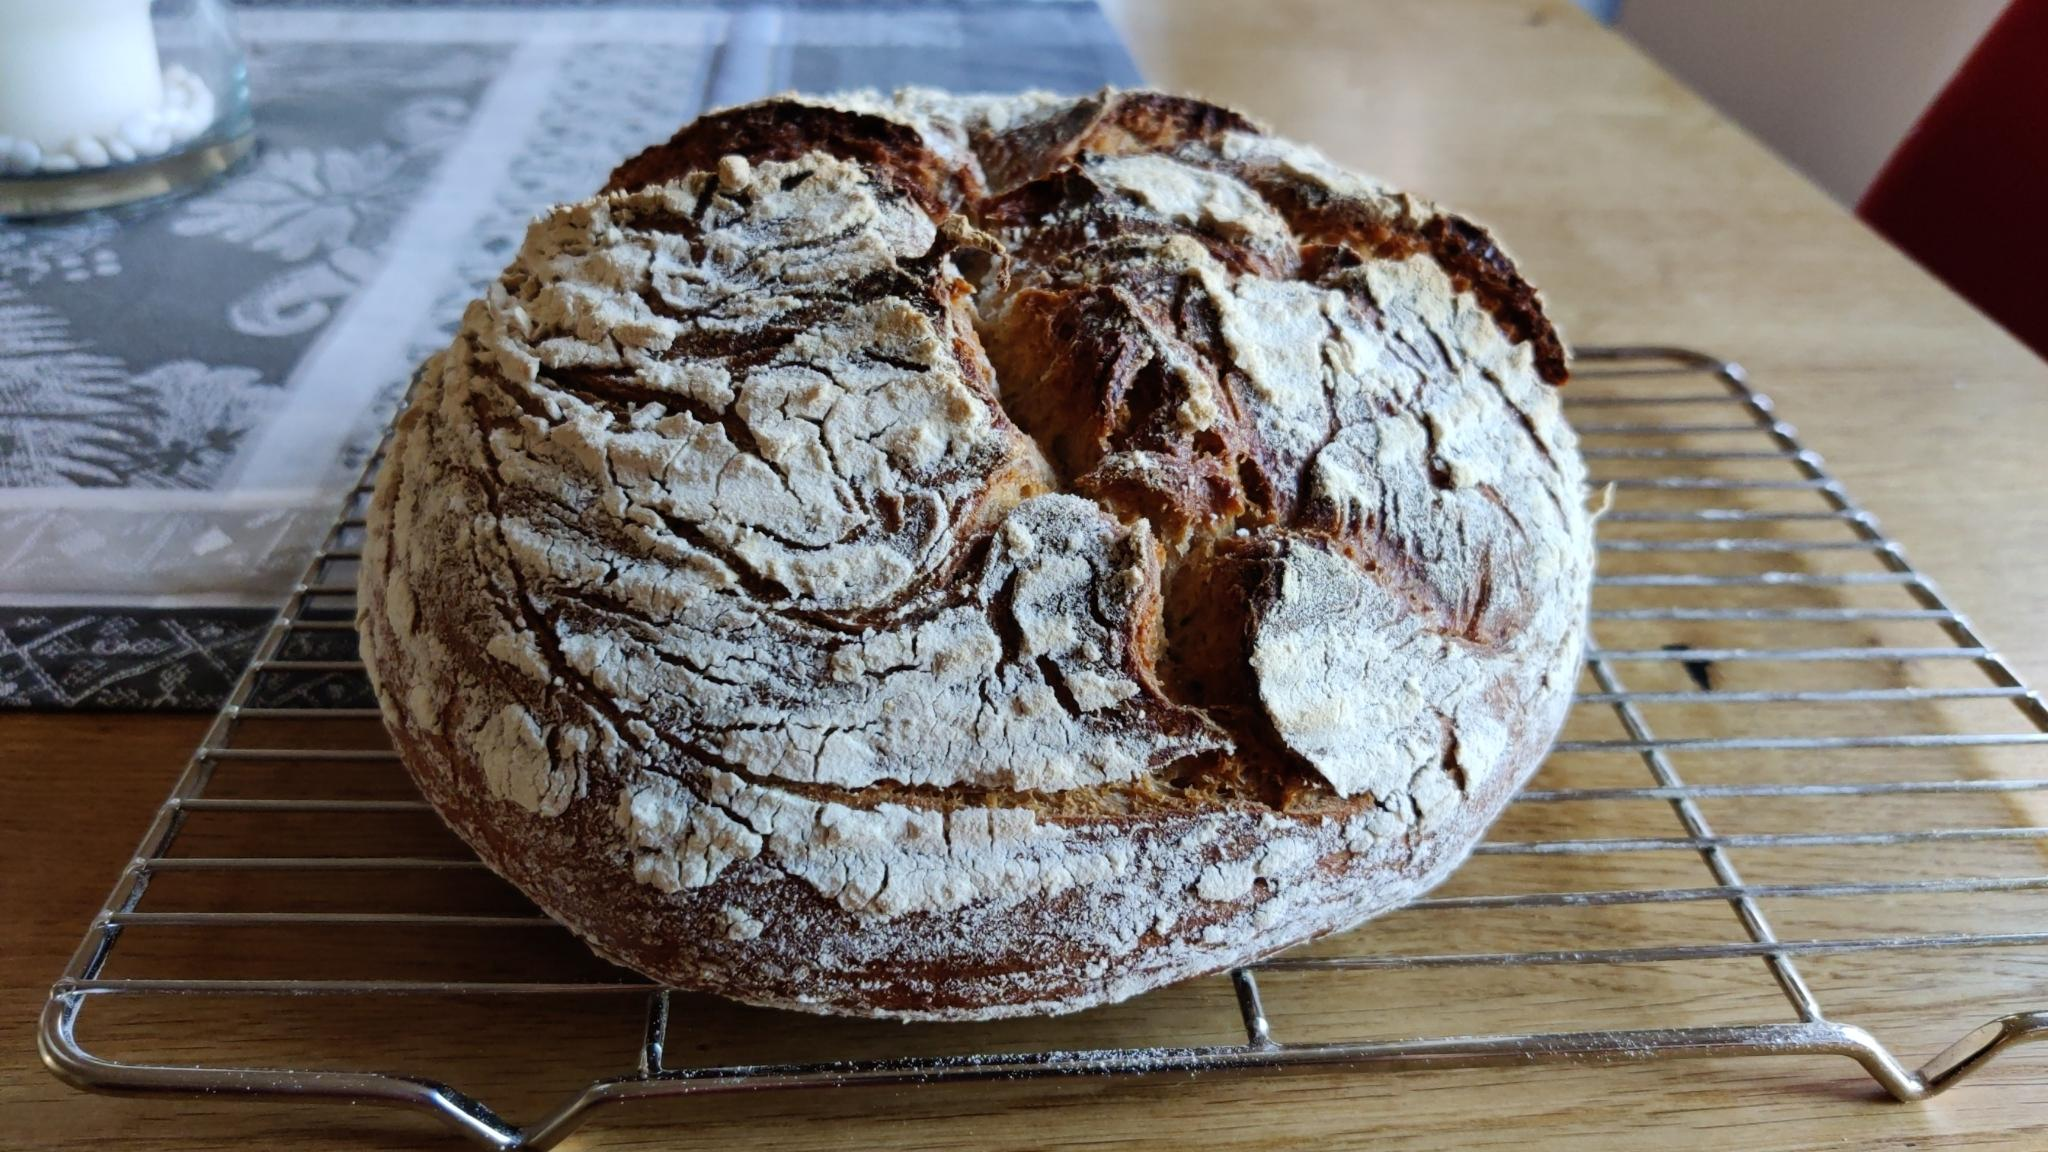
\includegraphics[width=0.7\linewidth]{Bilder/JulesSchwester}
%    \caption{Jules Schwester}
%    \label{fig:auffrischbrotJulesSchwester}
%\end{figure}

\subsection*{Zeitplan}
\begin{tabular}{ r @{ Uhr \phantom{bla} } l}
    \toprule
    \multicolumn{1}{c @{\phantom{ bla }}}{Zeit} & \multicolumn{1}{@{}l}{Aktion}   \\ \midrule
    00:00                                       & \Gls{Bruehstueck}               \\
    00:20                                       & \Gls{Fermentolyse}              \\
    01:00                                       & \Gls{Hauptteig}                 \\
    01:20                                       & \Gls{Stockgare}                 \\
    02:20                                       & \Gls{DehnenUndFalten}           \\
    03:20                                       & \Gls{DehnenUndFalten}           \\
    04:50                                       & \Gls{Formen}                    \\
    05:00                                       & \Gls{Stueckgare} im Kühlschrank \\
    17:30                                       & Vorheizen                       \\
    16:00                                       & \Gls{Backen}                    \\
    16:50                                       & fertig                          \\ \bottomrule
\end{tabular}
%
%
\subsection*{Alle Zutaten}
\begin{tabular}{r l}
           40 g & Altbrot geröstet                  \\
          120 g & heißer Kaffee                     \\
          150 g & Lievito Madre / Roggen Anstellgut \\
    250 / 225 g & kühles Wasser (LM / Roggen- ASG)  \\
          200 g & Weizenmehl Type 550               \\
          100 g & Weizenvolkorn                     \\
           50 g & Roggenvollkorn                    \\
           50 g & Roggen 1150                       \\
            3 g & Frischhefe                        \\
           10 g & Rübenkraut                        \\
           12 g & Salz
\end{tabular}\\


\section{Einfaches Auffrischbrot}  \index{Brot!Weizen}\index{Brot!Lievito Madre}\index{Auffrischbrot! Einfaches}
\begin{figure}[H]
    \centering
    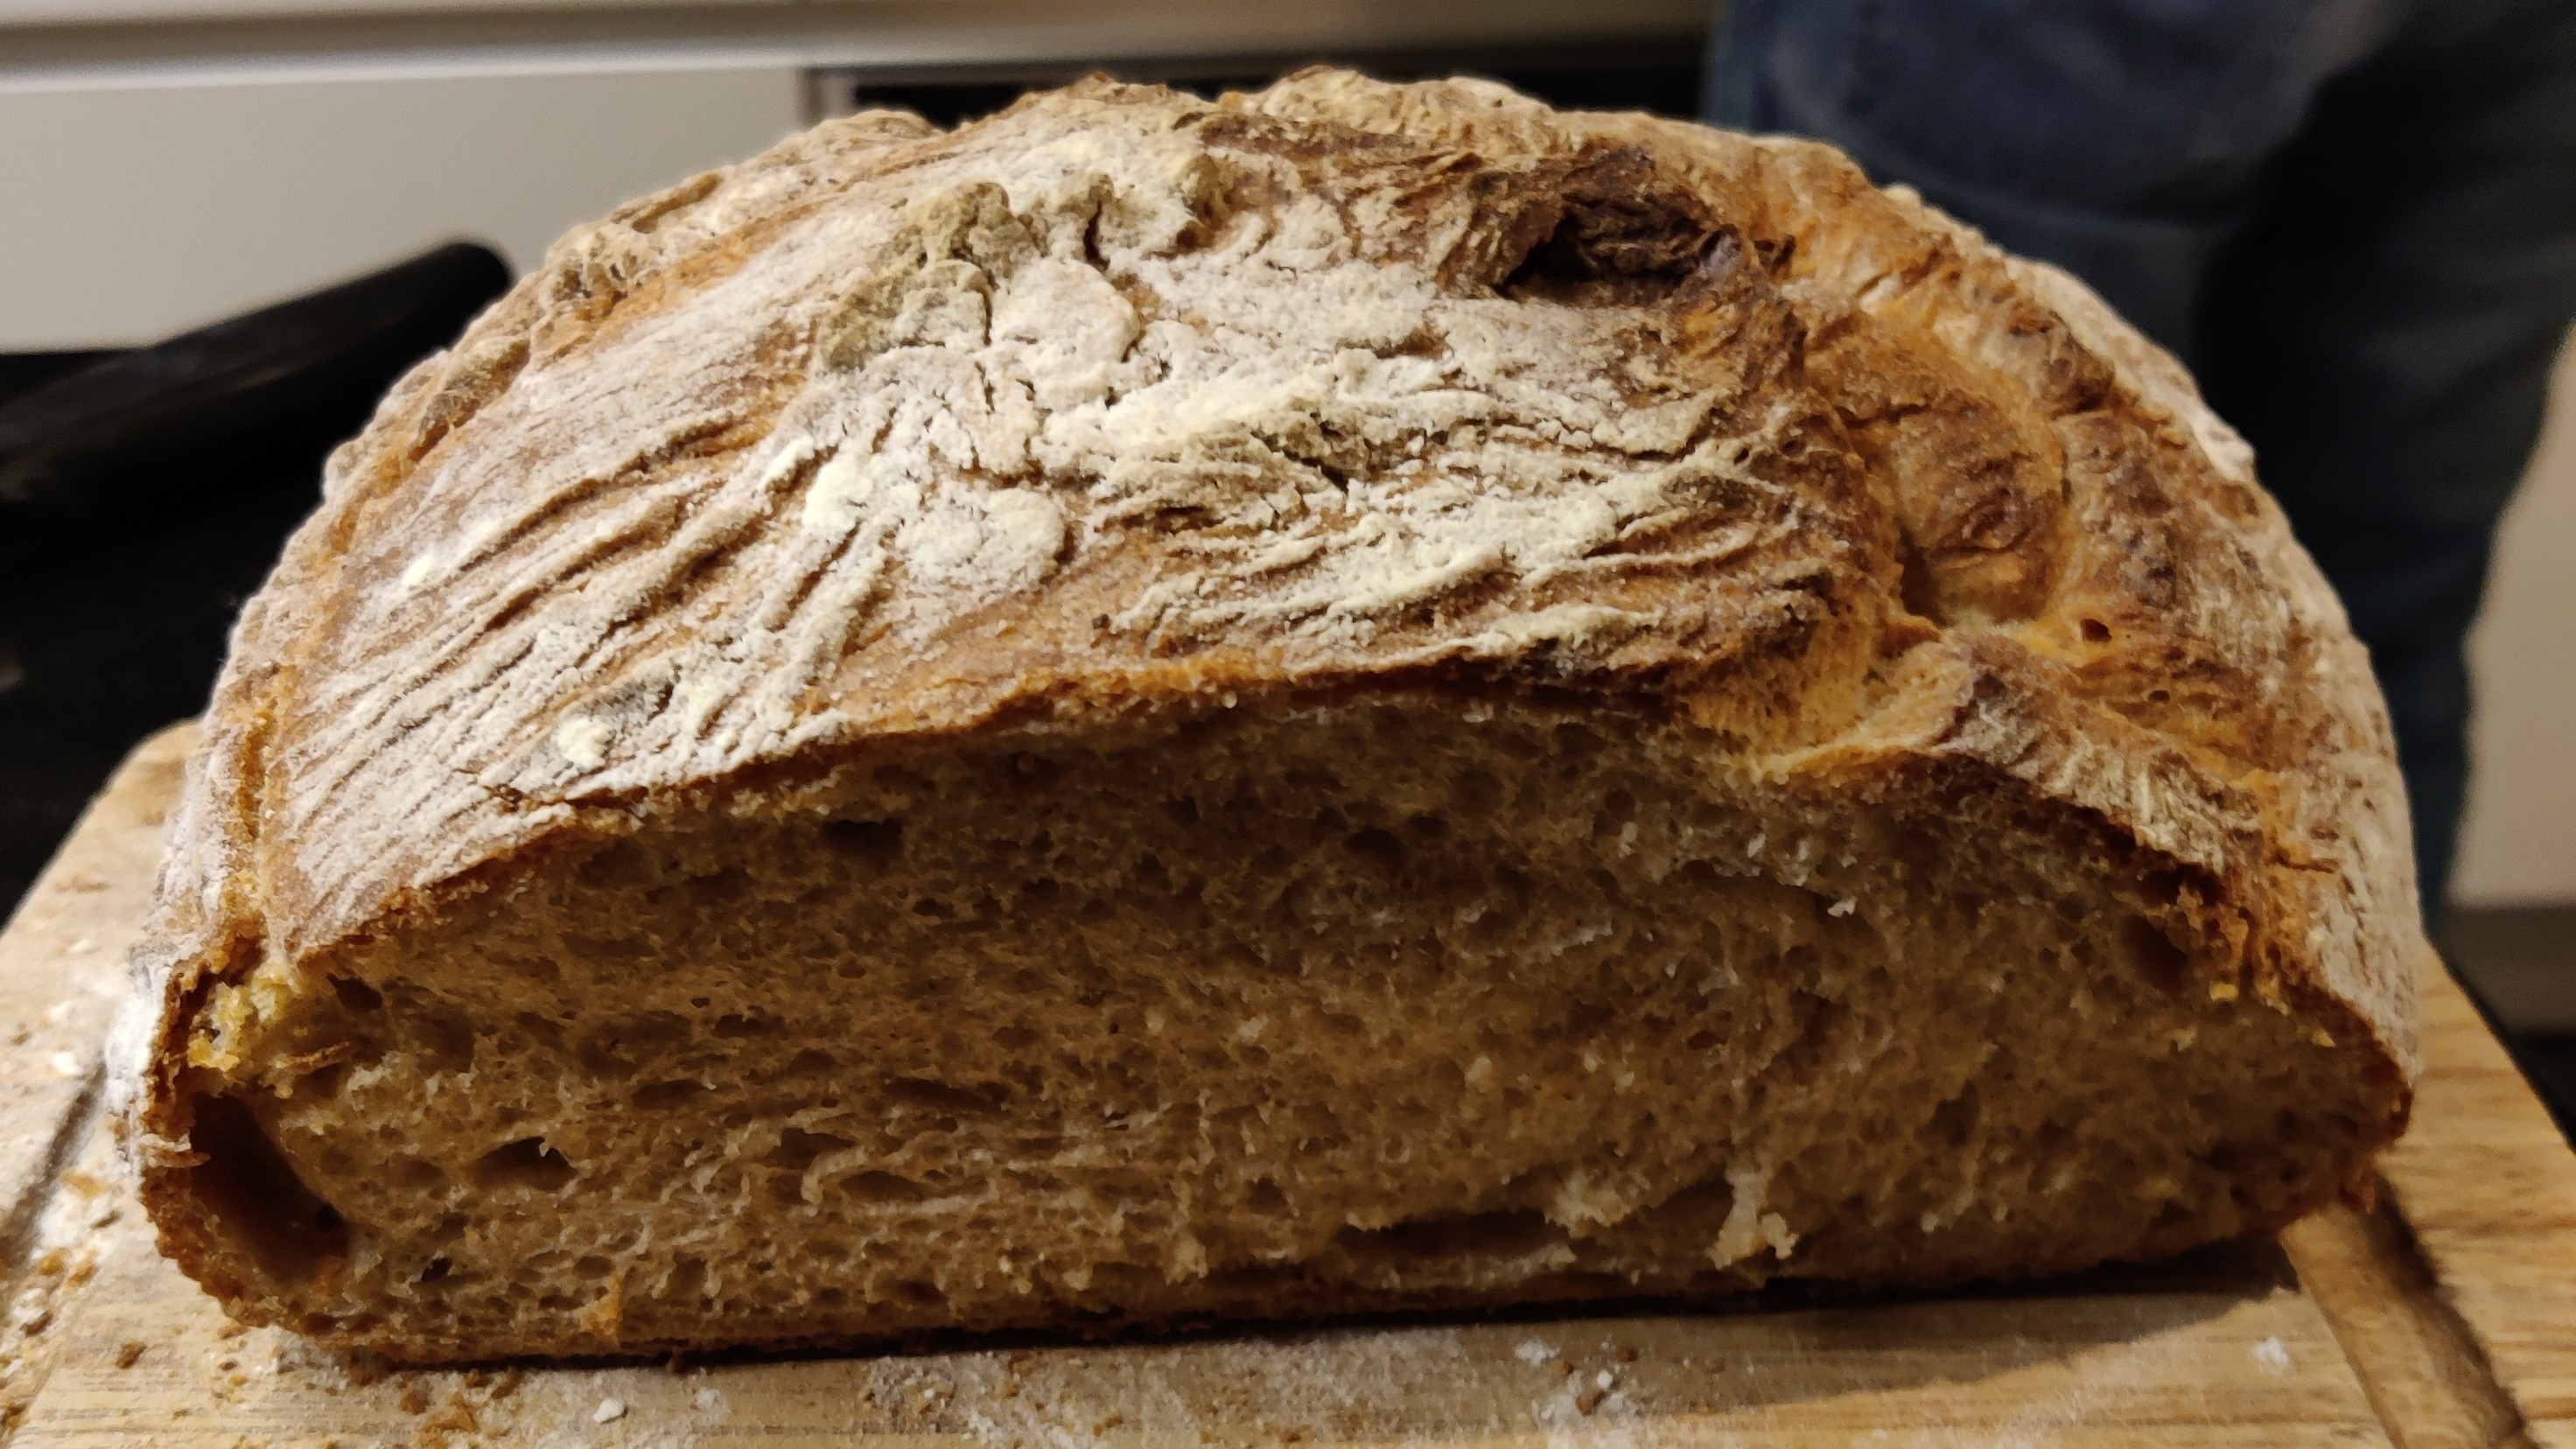
\includegraphics[width=0.7\linewidth]{Bilder/AuffrischbrotEinfach}
    \caption{Auffrischbrot Einfach}
    \label{fig:auffrischbroteinfach}
\end{figure}

\subsection*{Allgemeines}
\begin{tabular}{lrl}
    Gesamtzeit               &              ca. 5.30 & Stunden \\
    Fermentolyseteig mischen &                  0.00 & Uhr     \\
    Hauptteig zubereiten     &                  0.40 & Uhr     \\
    dehnen und falten        &                  1.40 & Uhr     \\
    Stockgare                &                  3.10 & Uhr     \\
    Backofen vorheizen       &                  4.20 & Uhr     \\
    formen + Stückgare       &                  4.50 & Uhr     \\
    backen                   &                  5.40 & Uhr     \\
    siehe                    & \cite[124]{SonjaBauer2021} &
\end{tabular}

\subsection*{Zutaten}

\subsubsection*{\Gls{Fermentolyse}}
\begin{tabular}{r l}
    120 g & Lievito-Madre-Anstellgut (+ 30 g Wasser)\\
    oder 150 g & Roggen ASG \\
    250 g & kühles Wasser\\
    250 g & Weizenmehl Type 550\\
    100 g & Weizenmehl Type 1050\\
    75  g & Vollkornmehl nach Wahl\\
\end{tabular}\\
Lievito Madre im Wasser auflösen, dann alles kurz, aber gründlich mischen und für 30 Minuten abgedeckt quellen lassen.


\subsubsection*{Hauptteig}
\begin{tabular}{r l}
    + & Fermentolyseteig                                      \\
    3 g & Frischhefe          \\
    10 g & Rübenkraut \\
    12 g & Salz                                                  \\
    %    10 g & Butter (oder Olivenöl)                                \\
    40 g & Wasser nach Bedarf (\Gls{Bassinage})                        \\
\end{tabular}\\


\subsection*{Zubereitung}
\begin{enumerate}
    \item [Teig] 
    %        \begin{itemize}
        %        \item Alle Zutaten (außer Salz + Bassinage) für 8–10 Minuten mit geringer Stufe kneten. Salz hinzufügen, für 3–5 Minuten mit höherer Stufe auskneten. Bei Bedarf noch bis zu
        %        40 g Wasser (Bassinage) mit einkneten.
        %\end{itemize}
        Alle Zutaten (außer Salz + Bassinage) für 8–10 Minuten mit geringer Stufe kneten. Salz hinzufügen, für 3–5 Minuten mit höherer Stufe auskneten. 
        
        Bei Bedarf noch bis zu 40 g Wasser (Bassinage) mit einkneten.
        \item [\Gls{Stockgare}]
        Den Teig in einer leicht geölten Schüssel oder Teigwanne bei Raumtemperatur abgedeckt etwa 3-4 Stunden bis zur guten Verdopplung reifen lassen, dabei nach 1 und 2 Stunden schonend dehnen und falten.
        \item [\Gls{Ballengare}]
        Den Teig auf einer bemehlten Arbeitsfäche locker rund wirken und abgedeckt für 20 Minuten mit dem Schluss nach unten entspannen lassen. 
        
        Danach rund wirken und mit dem Schluss nach unten in ein bemehltes Gärkörbchen geben.
        \item [\Gls{Stueckgare}]
        Abgedeckt für 90 Minuten bei Raumtemperatur (20−22 °C) reifen lassen.
        \item [Backen]
        Den Backofen rechtzeitig auf 250 °C Ober-/Unterhitze  vorheizen, zusammen mit einem Backstahl oder Backstein.
        
        Den Teigling aus dem Gärkörbchen stürzen und einschießen. Sofort schwaden. 
        
        Nach 10 Minuten den Dampf ablassen und die Temperatur auf 210° C reduzieren. Weitere 40 Minuten backen.
    \end{enumerate}


\section[Kornkasten]{Kornkasten \textmd{(siehe \cite[182]{SonjaBauer2021})}}  \index{Kastenbrot!Kornkaster}\index{Pollerbrot!Kornkasten}\index{Brot!Kastenbrot} \index{Buttermilch}


%\begin{figure}[H]
%%    \centering
%%    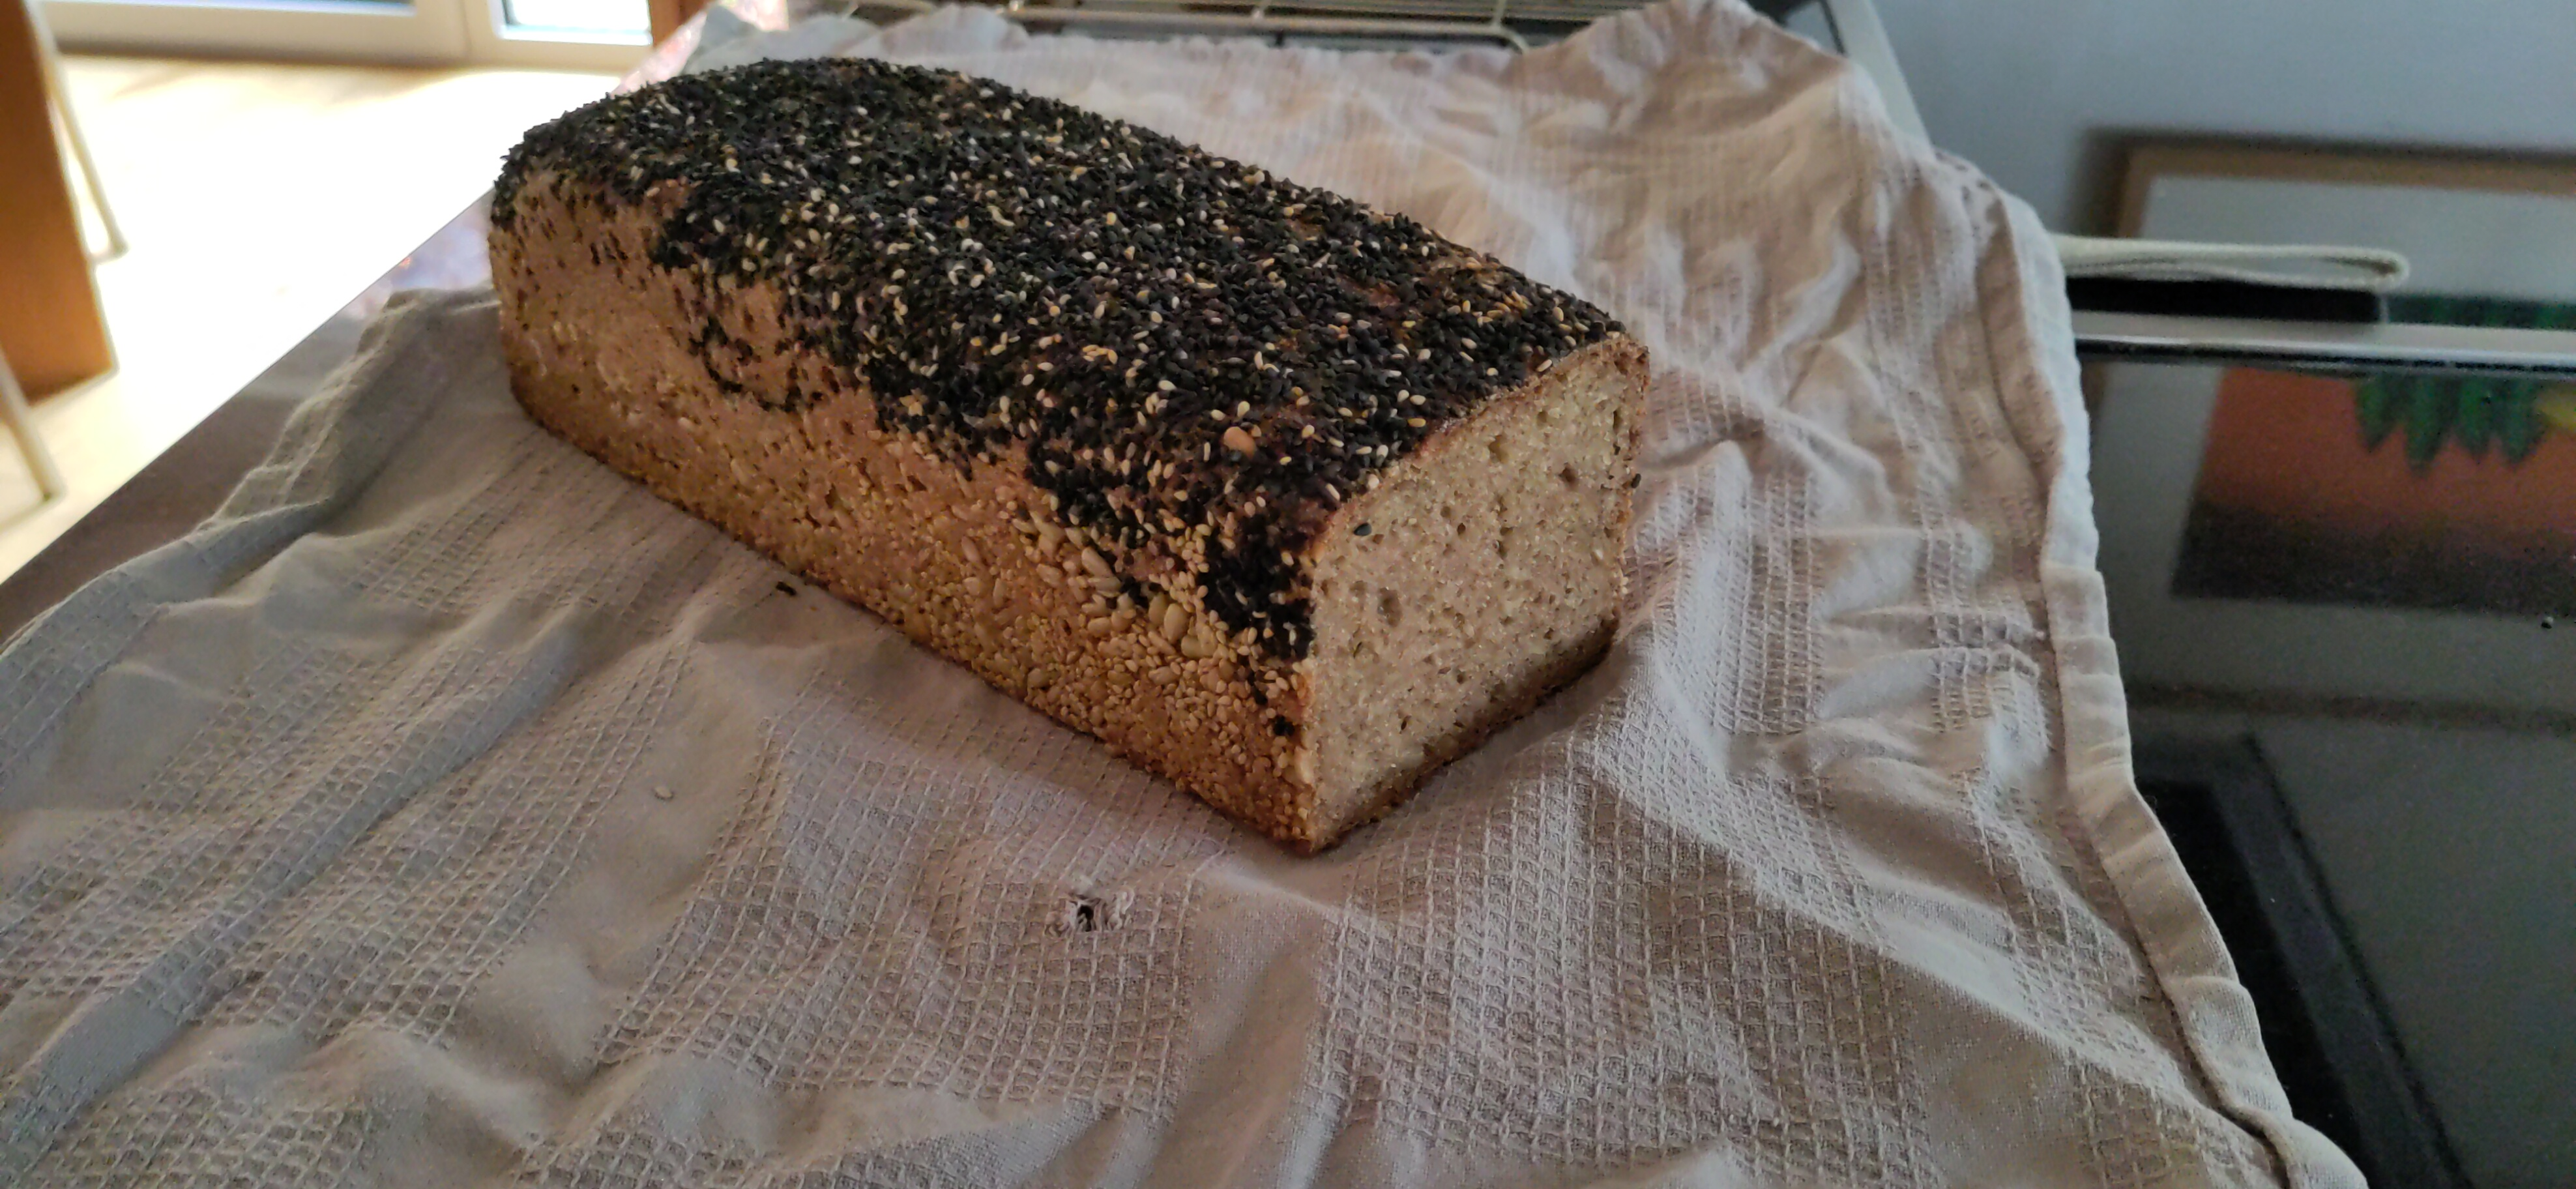
\includegraphics[width=0.7\linewidth]{Bilder/Vollkornprotz}
%%    \caption{Vollkornprotz mit schwarzem Sesam}
%%    \label{fig:vollkornprotz}
%\end{figure}

\subsection*{Zeitplan}
\begin{tabular}{ r @{ Uhr \phantom{bla} } l}
    \toprule
    \multicolumn{1}{c @{\phantom{ bla }}}{Zeit} & \multicolumn{1}{@{}l}{Aktion}   \\ \midrule
    00:00                                       & \Gls{Hauptteig}                 \\
    00:20                                       & \Gls{Stueckgare}     \\
    11:20                                       & Backen                          \\
    11:55                                       & Poller: fertig                  \\ 
    12:20                                       & Kasten: fertig                  \\ 
    \bottomrule
\end{tabular}
%
%
\subsection*{Zutaten}
%\subsubsection*{Alle Zutaten}
\begin{tabular}{r l}
    270  g & Wasser, 35° C         \\
    250  g & Buttermilch, kalt     \\
     25  g & Roggen-ASG (optional) \\
      1  g & Frischhefe            \\
    200  g & Weizenmehl T 1050     \\
    200  g & Roggenvollkornmehl    \\
    100  g & Roggenmehl 1150       \\
    100  g & Dinkelvollkornmehl    \\
      10 g & Rübensirup            \\
     25  g & Leinsamen, geschrotet \\
      14 g & Salz                  \\
      10 g & Rapsöl
\end{tabular}\\

\subsection*{Zubereitung}
\begin{enumerate}
    \item  [\Gls{Hauptteig}]  Wasser und Buttermilch mischen, Anstellgut (ASG) und Frischhefe darin auflösen.\\
    Danach alle Zutaten für den Hauptteig (außer Salz + Öl) hinzufügen und für 8–10     Minuten mit geringer Stufe kneten. In den letzten 2  Minuten Salz und Rapsöl zugeben.\\
    Kastenform oder 3 Weckgläser 0,75() gut einfetten und mit Roggenvollkornmehl oder gemahlenem Altbrot ausstreuen.\\
    Den Teig in Kastenform oder Gläser (Teigeinlage ca. 400 g) einfüllen, die Teigoberfläche mit einem angefeuchteten Teigschaber glattstreichen und mit Roggenvollkornmehl bestreuen. Kastenform bzw. Gläser sind gut zur Hälfte gefüllt.
    \item [\Gls{Stueckgare}] ZIEL: ca. 1 cm unter dem Rand. \\
    Abgedeckt für 10–12 Stunden bei Raumtemperatur zur Gare stellen. Der Teig soll etwa knapp den Rand der Form/Gläser erreichen.
    \item [Backen]  Backofen rechtzeitig mit einem Backstahl oder Backstein auf 230° C Ober-/Unterhitze vorheizen.\\
    Einschießen und wenig schwaden. Für insgesamt etwa 60 Minuten (Kastenbrot) bzw. 35-40 Minuten (Pollerbrote) backen.\\
    Nach 10 Minuten die Temperatur auf 200° C reduzieren. Nach dem Backen aus der Form lösen und nochmal für 10 Minuten bei leicht geöffneter Backofentür zurück in den Ofen geben. 
\end{enumerate}


\chapter{Hefe}
\section{Ciabatta}  \index{Brot!Weizen}\index{Brot!Hefe}\index{Ciabatta}
\subsection*{Allgemeines}
\begin{tabular}{lrl}
    Gesamtzeit          & ca. 17 & Stunden \\
    Vorteig erstellen   &      5 & Minuten \\
    Vorteig ruhen       &     12 & Stunden \\
    Hauptteig erstellen &     10 & Minuten \\
    1. Gehzeit          &      3 & Stunden \\
    Backzeit            &     30 & Minuten
\end{tabular} 
\subsection*{Zutaten}
\begin{tabular}{lrr}
    Hefe               &   2 &  g \\
    Zucker             &   1 & TL \\
    Weizenmehl Tipo 0 &  300 &  g \\
    Hartweizenmehl     &  50 &  g \\
    Wasser             & 225 & ml \\
    Salz               &   1 & TL \\
    Olivenöl           &   4 & EL
\end{tabular} 


\subsection*{Zubereitung}

\begin{enumerate}
    \item Hefe, Zucker, Weizenmehl und 125 ml Wasser glatt rühren und abgedeckt ca. 12 Std. warm ruhen lassen. 
    \item Restliche trockene Zutaten mit dem Vorteig grob mischen. 100 ml
    warmes Wasser mit dem Öl zum Mehl geben und ca. 5 Min. kräftig
    rühren, bis sich der Teig vom Schüsselrand löst. Kein Wasser zugeben. Teig nach der ersten und zweiten Stunde falten \todo{Bilder einfügen} und dann jeweils stehen lassen, Eine weitere Stunde in der Schüssel ruhen lassen.
    
    \item Den Teig auf Backpapier stürzen, zu einem länglichen Laib auseinander ziehen und mit einer Haube abdecken. 1 Std. ruhen lassen.\\
    Den Backofen auf 240° vorheizen, wenn vorhanden mit Backstahl oder Backstein. Das Brot
    mit Wasser besprühen und mit Mehl bestreuen. Etwas Wasser mit in den Ofen und das Brot auf der mittleren Schiene ca.15 Min. backen. Danach die Temperatur auf 210° reduzieren und das Brot in weiteren 15 Min. fertig backen.
    
\end{enumerate}   


\section[Dinkel-Bauernkruste]{Dinkel-Bauernkruste \textmd{(siehe \cite[170]{SonjaBauer2021})}}  \index{Brot!Dinkel-Bauernkruste} \index{Magerquark} \index{Brot!Dinkel}

\subsection*{Zeitplan}
\begin{tabular}{ r @{ Uhr \phantom{bla} } l}
    \toprule
    \multicolumn{1}{c @{\phantom{ bla }}}{Zeit} & \multicolumn{1}{@{}l}{Aktion} \\ \midrule
    00:00                                       & \Gls{Autolyse}                \\
    00:30                                       & \Gls{Hauptteig}               \\
    00:50                                       & \Gls{Stockgare}(20- 22 Grad)  \\
    01:35                                       & \Gls{DehnenUndFalten}         \\
    02:20                                       & \Gls{DehnenUndFalten}         \\
    11:50                                       & \Gls{Formen}                  \\
    12:00                                       & \Gls{Stueckgare}              \\
    13:00                                       & Vorheizen                     \\
    13:30                                       & \Gls{Backen}                  \\
    14:15                                       & fertig                        \\ \bottomrule
\end{tabular}

\subsection*{Alle Zutaten}
\begin{tabular}{r l}
    280 g & Wasser, kühl       \\
    0,8 g & Acerola-Pulver     \\
    100 g & Magerquark, kalt   \\
    350 g & Dinkelmehl  630    \\
      5 g & Flohsamenschalen   \\
    150 g & Dinkelvollkornmehl \\
      1 g & Hefe               \\
     10 g & Honig              \\
     12 g & Salz               \\
     10 g & Butter             \\
     20 g & Bassinage
\end{tabular}\\

\subsection*{Zubereitung}
    \subsubsection*{\GLS{Autolyse}} 
    \begin{tabular}{r l}
        280 g & Wasser, kühl       \\
        0,8 g & Acerola-Pulver     \\
        100 g & Magerquark, kalt   \\
        350 g & Dinkelmehl  630    \\
          5 g & Flohsamenschalen   \\
        150 g & Dinkelvollkornmehl
    \end{tabular} 
    
         Acerola in dem Wasser auflösen. Danach alles kurz,aber gründlich mischen und für 30 Minuten abgedeckt quellen lassen.
    
    \subsubsection*{\Gls{Hauptteig}}  
    \begin{tabular}{r l}
           + & Autolyse  \\
         1 g & Hefe      \\
        10 g & Honig     \\
        12 g & Salz      \\
        10 g & Butter    \\
        20 g & Bassinage
    \end{tabular}
    
    Alle Zutaten (außer Salz + Butter + Bassinage) für 8–10 Minuten mit geringer Stufe kneten. Salz und Butter zugeben, für 1–2 Minuten mit höherer Stufe auskneten. Dabei bei Bedarf bis zu 20 g Wasser (Bassinage) mit einkneten.
    
    \subsubsection*{\Gls{Stockgare}}
    Abgedeckt für 10–12 Stunden bei Raumtemperatur zur Gare stellen. Nach 45 und 90 Minuten dehnen und falten.
    
    \subsubsection*{\GLS{Formen}}
    Auf der bemehlten Arbeitsfläche schonend rund wirken und mit dem Schluss nach unten in ein bemehltes Gärkörbchen geben.
    
    \subsubsection*{\Gls{Stueckgare}} 
    Abgedeckt für 10–12 Stunden bei warmer Raumtemperatur (22–24° C) zur Gare stellen. Der Teig soll etwa knapp den Rand der Form erreichen.
    \subsubsection*{\Gls{Backen}}
    Backofen rechtzeitig auf 250° C Ober–/Unterhitze vorheizen.\\
    Teigling aus dem Gärkörbchen stürzen und einschießen. Sofort schwaden und für insgesamt 40–50
    Minuten backen. Nach 10 Minuten den Dampf ablassen und die Temperatur auf 210° C reduzieren.
    

















 
 
 

 









